% !TeX spellcheck = cs_CZ
% file: kap_mag_obvody.tex
%{\tikzset{external/prefix={tikz/TEO/}}
% \tikzset{external/figure name/.add={ch06_}{}}
%==================== Kapitola: Magnetické obvody =================================================
\setchaptertoc
\chapter{Magnetické obvody}\label{teo:IchapV}

  
  Z topologického hlediska může být magnetický obvod \textbf{spojitý} nebo \textbf{diskrétní}. Tato 
  kapitola je věnována především obvodům diskrétním, tedy takovým, které obsahují feromagnetické 
  jádro s velikou permeabilitou. Tím je zajištěno, že prakticky veškerý tok prochází prostorově 
  ohraničenou, tj. diskrétní, cestou, která je vymezena geometrií jádra.
  
  \section{Tříděni magnetických obvodů}\label{teo:IchapVsecI}
    Podle tvaru magnetizační charakteristiky \(\Psi=\Psi(i)\), tedy podle tvaru funkční závislosti 
    spřaženého; toku na proudu, je možno magnetické obvody třídit na
    \begin{enumerate}[noitemsep]
      \item \textbf{lineární},
      \item \textbf{nelineární}.
    \end{enumerate}
    
    \textbf{Parametrickým obvodem} rozumíme případ, kdy je tok \(\Psi\) funkčně závislý kromě 
    proudu na dalším fyzikálním parametru \(p\), např. na délce vzduchové mezery, na teplotě atd. 
    Zřejmě se mohou vyskytovat všechny \emph{čtyři kombinace} uvedených dvou vlastností. Tyto čtyři 
    možnosti jsou zachyceny na obr. \ref{teo:fig001}, přičemž hysterezi na obr. \ref{teo:fig001c} 
    je nutno chápat jako zvláštní a složitější případ nelinearity na obr. \ref{teo:fig001b}. V 
    následujících kapitolách budou všechny čtyři případy (kromě hystereze) analyzovány matematicky. 
    Cílem analýzy bude \emph{výpočet indukovaného napětí} cívky v libovolně složité situaci, tedy 
    především v případě cívky nelineární a navíc parametrické. Umění vypočíst indukované napětí v 
    libovolné fyzikální situaci je totiž základem pro vytváření \emph{matematických modelů} 
    transformátorů a všech elektromechanických měničů energie (motorů, pracovních elektromagnetů, 
    magnetických snímačů polohy atd.).
 
  
    \begin{figure}[ht!]  %\ref{teo:fig001}
      \centering
      \subcaptionbox{\label{teo:fig001a}}{\luafigure[0.3]{teo_fig001a.jpg}}
      \subcaptionbox{\label{teo:fig001b}}{\luafigure[0.3]{teo_fig001b.jpg}} \\
      \subcaptionbox{\label{teo:fig001c}}{\luafigure[0.3]{teo_fig001c.jpg}}
      \subcaptionbox{\label{teo:fig001d}}{\luafigure[0.3]{teo_fig001d.jpg}} \\
      \subcaptionbox{\label{teo:fig001e}}{\luafigure[0.3]{teo_fig001e.jpg}} 
      \caption{Třídění magnetických obvodů: a) lineární, b) nelineární, c) nelineární s hysterezi,
               d) lineární parametrický, e) nelineární parametrický.
               (\cite[s.~150]{Patocka4})}
      \label{teo:fig001}
    \end{figure}
    
  \section{Lineární magnetický obvod}\label{teo:IchapVsecII}
    Je-li magnetický obvod lineární podle obr. \ref{teo:fig001}, pak musí platit přímá úměra mezi 
    spřaženým tokem a proudem:
    \begin{equation}\label{TEO:eq001}
      \Psi    = LI, \quad\text{resp.}\quad
      \Psi(t) = Li(t).
    \end{equation}
    Konstanta úměrnosti se nazývá indukčnost \(L\). Rovnice \(\Psi=LI\) má současně význam 
    \textbf{statické definici indukčnosti}. Je však vidět, že přímá úměra platí podle rovnice 
    \(\Psi(t) = Li(t)\) i \textbf{dynamicky}, pro okamžité hodnoty veličin měnících se 
    \emph{libovolně} v čase.
    
    \begin{figure}[ht!]  %\ref{teo:fig002}
      \centering
      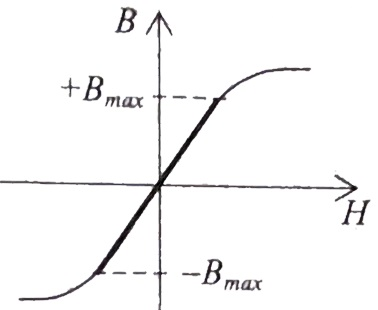
\includegraphics[width=0.5\linewidth]{teo_fig002.jpg}
      \caption{Linearizovaný magnetizační obvod
              (\cite[s.~151]{Patocka4})}
      \label{teo:fig002}
    \end{figure}
    
    V technické praxi je možno považovat i feromagnetický obvod za \emph{přibližně} lineární, 
    pohybuje-li se pracovní bod pouze v lineární oblasti magnetizační charakteristiky podle obr. 
    \ref{teo:fig002}. Namísto \emph{absolutní} magnetizační charakteristiky \(\Psi = \Psi(I)\) je 
    výhodnější používat \emph{relativní normovanou} charakteristiku  \(B= B(H)\), která není 
    závislá na geometrických rozměrech magnetického obvodu, a proto umožňuje vzájemně porovnávat 
    vlastnosti různých materiálů.

    \subsection{Hopkinsonův zákon}
      Zanedbáme-li rozptylový tok jdoucí okolními vzdušnými ces\-tami, pak lze magnetický obvod na 
      obr. \ref{teo:fig003} považovat za diskrétní. Diskrétním obvodem rozumíme obvod, v němž je 
      cesta magnetického toku\(\Phi\) ostře vytyčena a ohraničena v prostoru. Za diskrétní obvod 
      lze v technické praxi považovat všechna feromagnetická jádra jednodušších tvarů, 
      feromagnetikum však nesmí být v \textbf{přesyceném} stavu; pak totiž prudce klesá jeho 
      permeabilita (tj. měrná magnetická vodivost)
      
      \begin{figure}[ht!]  %\ref{teo:fig003}
        \centering
        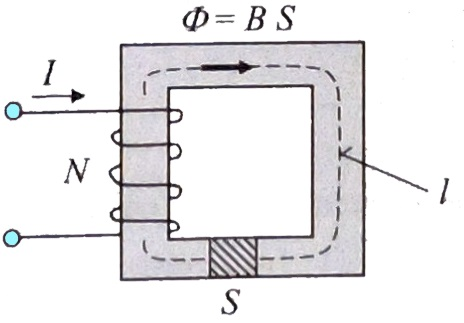
\includegraphics[width=0.5\linewidth]{teo_fig003.jpg}
        \caption{Lineární diskrétní magnetický obvod.
                (\cite[s.~151]{Patocka4})}
        \label{teo:fig003}
      \end{figure}
      
      Má-li magnetický obvod na obr. \ref{teo:fig003} po celé délce \(l\) konstantní průřez \(S\) i 
      permeabilitu, pak je \emph{homogenní}. V tom případě lze zavést následující 
      magneticko-elektrické analogie:
      \begin{alignat}{3}
       \shortintertext{magnetické napětí (\emph{\uv{ampérzávity}}):}
        & U_m = NI = Hl        \quad && \text{ } \qquad
           && [A; A/m, m],  \label{TEO:eq002a}  \\
        \shortintertext{magnetický tok (\emph{\uv{magnetický proud}}):} 
        & I_m\equiv\Phi = BS \quad && \text{ } \qquad 
           && [Wb; T. m^2], \label{TEO:eq002b}  \\
        \shortintertext{magnetická vodivost:}
        & \boxed{\lambda = \frac{I_m}{U_m}} \quad && \text{ } \qquad 
           && [H; Wb, A].   \label{TEO:eq002c} 
      \end{alignat}
      Rovnice (\ref{TEO:eq002c}) se nazývá \textbf{Hopkinsonův  zákon}\footnote{John Hopkinson 
      (\num{1849}-\num{1898}), britský fyzik a inženýr, člen Královské společnosti, v období 1890 - 
      1896 prezident IEE. Vynálezce trojfázové napájecí soustavy (patent z r. 1882). Působil na 
      King's College v Londýně a také jako ředitel Laboratoří Siemens.}. Jedná se o analogii 
      \emph{Ohmova zákona}. Dosadíme-li pravé strany rovnic (\ref{TEO:eq002a}) a (\ref{TEO:eq002b}) 
      do (\ref{TEO:eq002c}), dospíváme k výrazu
      \begin{equation}  \label{TEO:eq003}
        \lambda_m = \frac{BS}{Hl} = \mu\frac{S}{l}
      \end{equation}
      Podle analogie s elektrickou vodivosti vidíme, že magnetická permeabilita \(\mu\) má význam 
      \textbf{měrné magnetické vodivosti} daného materiálu, viz obr. \ref{teo:fig004}. Z rovnice 
      (\ref{TEO:eq003}) plyne
      \begin{equation}  \label{TEO:eq004}
        \boxed{\mu = \frac{B}{H} = \mu_r\mu_0} \qquad [H/m; T, A/m]
      \end{equation}
      kde \(\mu_r\) je \textbf{relativní permeabilita materiálu}, vztažená k permeabilitě vakua.
      \begin{figure}[ht!] %\ref{teo:fig004}
        \centering
        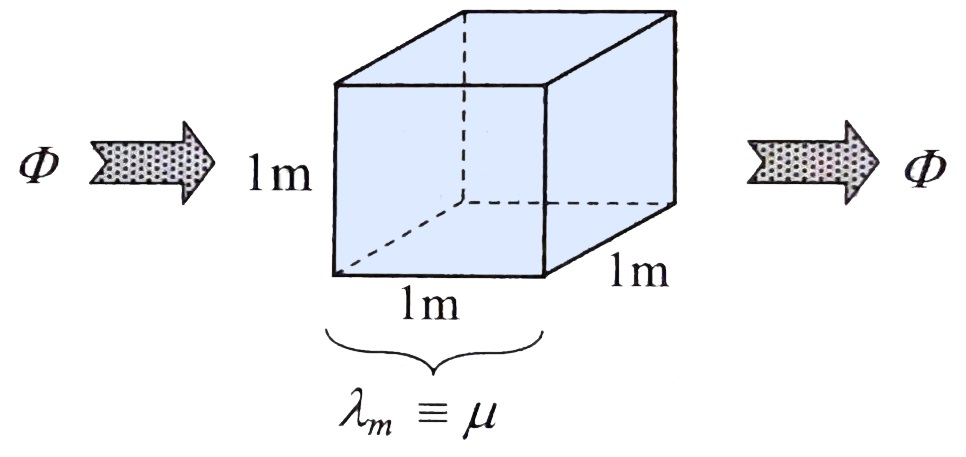
\includegraphics[width=0.6\linewidth]{teo_fig004.jpg}
        \caption{Permeabilita neboli měrná magnetická vodivost materiálu je magnetická vodivost 
                 krychle o straně 1 m.
                 (\cite[s.~152]{Patocka4})}
        \label{teo:fig004}
      \end{figure}

    \subsection{Indukčnost lineárního diskrétního magnetického obvodu}
      Dosadíme-li do Hopkinsonova zákona (\ref{TEO:eq002c}), psaného ve tvaru \(U_m\lambda_m=I_m\), 
      rovnice (\ref{TEO:eq002a}) a (\ref{TEO:eq002b}), získáme vztah
      \begin{equation}  \label{TEO:eq005}
        NI\lambda_m = \Phi\qquad\mid \cdot N
      \end{equation}
      Po vynásobení obou stran rovnice počtem závitů \(N\) a následným porovnáním se vztahem \(\Psi 
      = LI\) získáme relaci
      \begin{equation}  \label{TEO:eq006}
        \underbrace{N^2\lambda_m}_L I = N\Phi \cong\Psi = LI.
      \end{equation}
      Porovnáním prvního a posledního výrazu ve složené relaci (\ref{TEO:eq006}) dospíváme ke 
      zjištění, že indukčnost lineárního diskrétního magnetického obvodu musí mít velikost
      \begin{equation}  \label{TEO:eq007}
        \boxed{L = N^2\lambda_m = N^2\mu\frac{S}{l}.}
      \end{equation}
      U feritových jader bývá zvykem modifikovat rovnici (\ref{TEO:eq007}) do praktického tvaru 
      \begin{equation}  \label{TEO:eq008}
        \boxed{L = N^2\lambda_m = N^2A_L.} \qquad [nH; -, nH/\text{závit}^2],
      \end{equation}
      kde \(A_L\) je tzv. \textbf{konstanta jádra} uváděná výrobcem. Konstanta má význam magnetické 
      vodivosti jádra, ale vyjádřené v praktických jednotkách.

    \subsection{Elektromagnetický návrh lineárního diskrétního magnetického obvodu}
       Porovnáním pravých stran rovnic (\ref{vol02:TEO:eq092}), (\ref{TEO:eq001}) získáme vztah
      \begin{equation}  \label{TEO:eq009}
        \Psi(t) \cong N\Phi(t) = Li(t),
      \end{equation}
      který lze přepsat do tvaru
      \begin{equation}  \label{TEO:eq010}
        \boxed{NB(t)S = Li(t)}
      \end{equation}
      Velmi důležitá rovnice (\ref{TEO:eq010}) slouží pro přímý návrh všech tlumivek, 
      transformátorů a elektrických strojů s feromagnetickým jádrem a bude využita v příslušných 
      kapitolách.
      
    \subsection{Hopkinsonovy činitele rozptylu}
      Týkají se diskrétního magnetického \emph{obvodu} se dvěma nebo více vinutími, tedy 
      \emph{transformátoru} nebo \emph{motoru}. Situace je znázorněna na obr. \ref{teo:fig005}.
      
      Hopkinsonův činitel rozptylu \(\upsilon\) je obecně definován 
      \begin{equation}  \label{TEO:eq013}
        \upsilon = \frac{\text{celkový tok \(\Phi_{11}\) vyslaný vysílací cívkou}}{\text{tok 
        \(\Phi_{21}\) procházející přijímací cívkou}},
      \end{equation}
      kde \(\upsilon\geqq1\) vždy.
      
      \begin{figure}[ht!]  %\ref{teo:fig005}
        \centering
        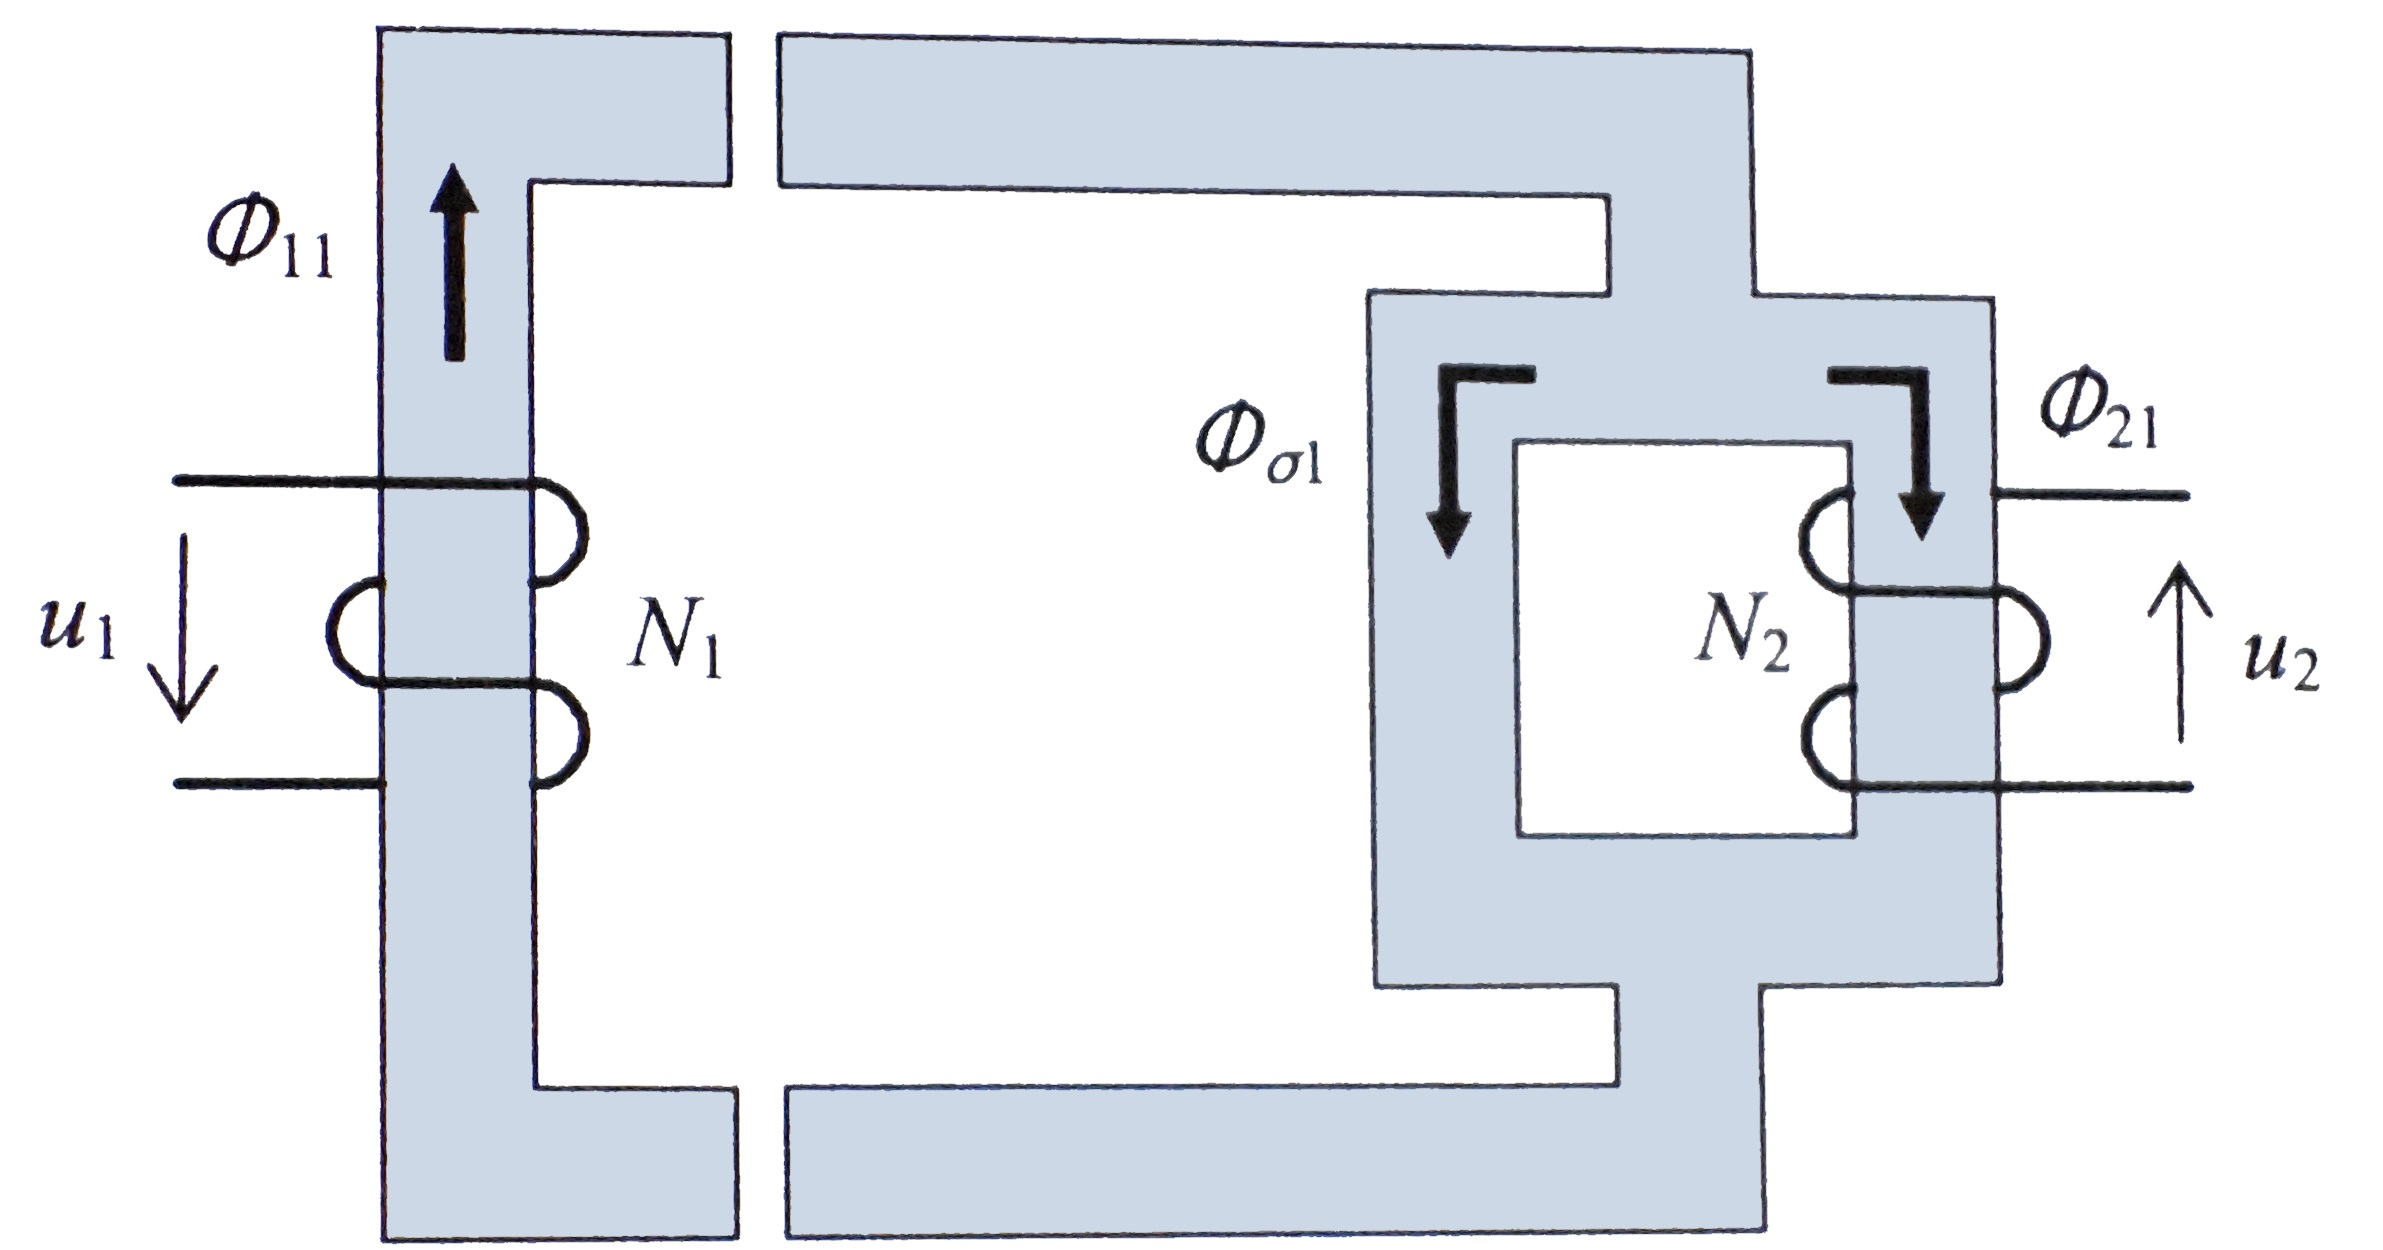
\includegraphics[width=0.8\linewidth]{teo_fig005.jpg}
        \caption{K definici Hopkinsonova činitele rozptylu.
                (\cite[s.~153]{Patocka4})}
        \label{teo:fig005}
      \end{figure}
      Vidíme, že při určování Hopkinsonova činitele musí být sekundární (přijímací) cívka ve stavu 
      \emph{elektricky naprázdno}, což odpovídá stavu \emph{magneticky nakrátko} (její sloupek o 
      nekonečné magnetické vodivosti se chová vůči toku \(\Phi_{21}\), jako \emph{magnetický 
      zkrat}). Kdybychom totiž naopak sekundární cívku elektricky \emph{zkratovali}, bude na ní 
      \emph{nulové} napětí, tedy i\emph{ nulový integrál z napětí}, tedy i nulový tok. Tento stav 
      lze popsat jako stav \emph{elektricky nakrátko}, což odpovídá stavu \emph{magneticky 
      naprázdno} (sloupek zkratované „supravodivé“ sekundární cívky se chová vůči toku \(\Phi\) i 
      jako dokonalý \textbf{magnetický izolant}). Podobně lze určit Hopkinsonův činitel rozptylu v 
      obráceném směru, zaměníme-li navzájem role obou cívek. Podrobnější rozbor Hopkinsonových 
      činitelů rozptylu, především jejich matematický vztah k \textbf{činiteli magnetické vazby} 
      \(k\), bude uveden v kapitole o transformátoru \ref{ES:kap_teorie_trafa}.
       
    \subsection{Výpočet indukovaného napětí}
      Magnetizační charakteristika lineárního magnetického obvodu má tvar \emph{přímky} dané rovnicí
      \begin{equation}\label{TEO:eq014}
        \Psi = L[i], \qquad\text{resp.}\qquad \Psi[i(t)] = Li(t).
      \end{equation}
      Z formálního matematického pohledu lze na magnetizační charakteristiku \(\Psi = L[i]\) 
      pohlížet jako na \emph{složenou} funkci dynamickou \(\Psi[i(t)] = Li(t)\), kde hranatými 
      závorkami je vyznačena \emph{vnější} statická funkce proudu a závorkami kulatými je vyznačena 
      \emph{vnitřní} dynamická funkce času. Z rovnic (\ref{TEO:eq014}) lze získat \textbf{inverzní 
      magnetizační charakteristiku} ve tvaru
      \begin{equation}\label{TEO:eq015}
        i = \frac{\Psi}{L}, \qquad\text{resp.}\qquad i(t) = \frac{\Psi(t)}{L}.
      \end{equation}
      
      \begin{figure}[ht!]  %\ref{teo:fig006}
        \centering
        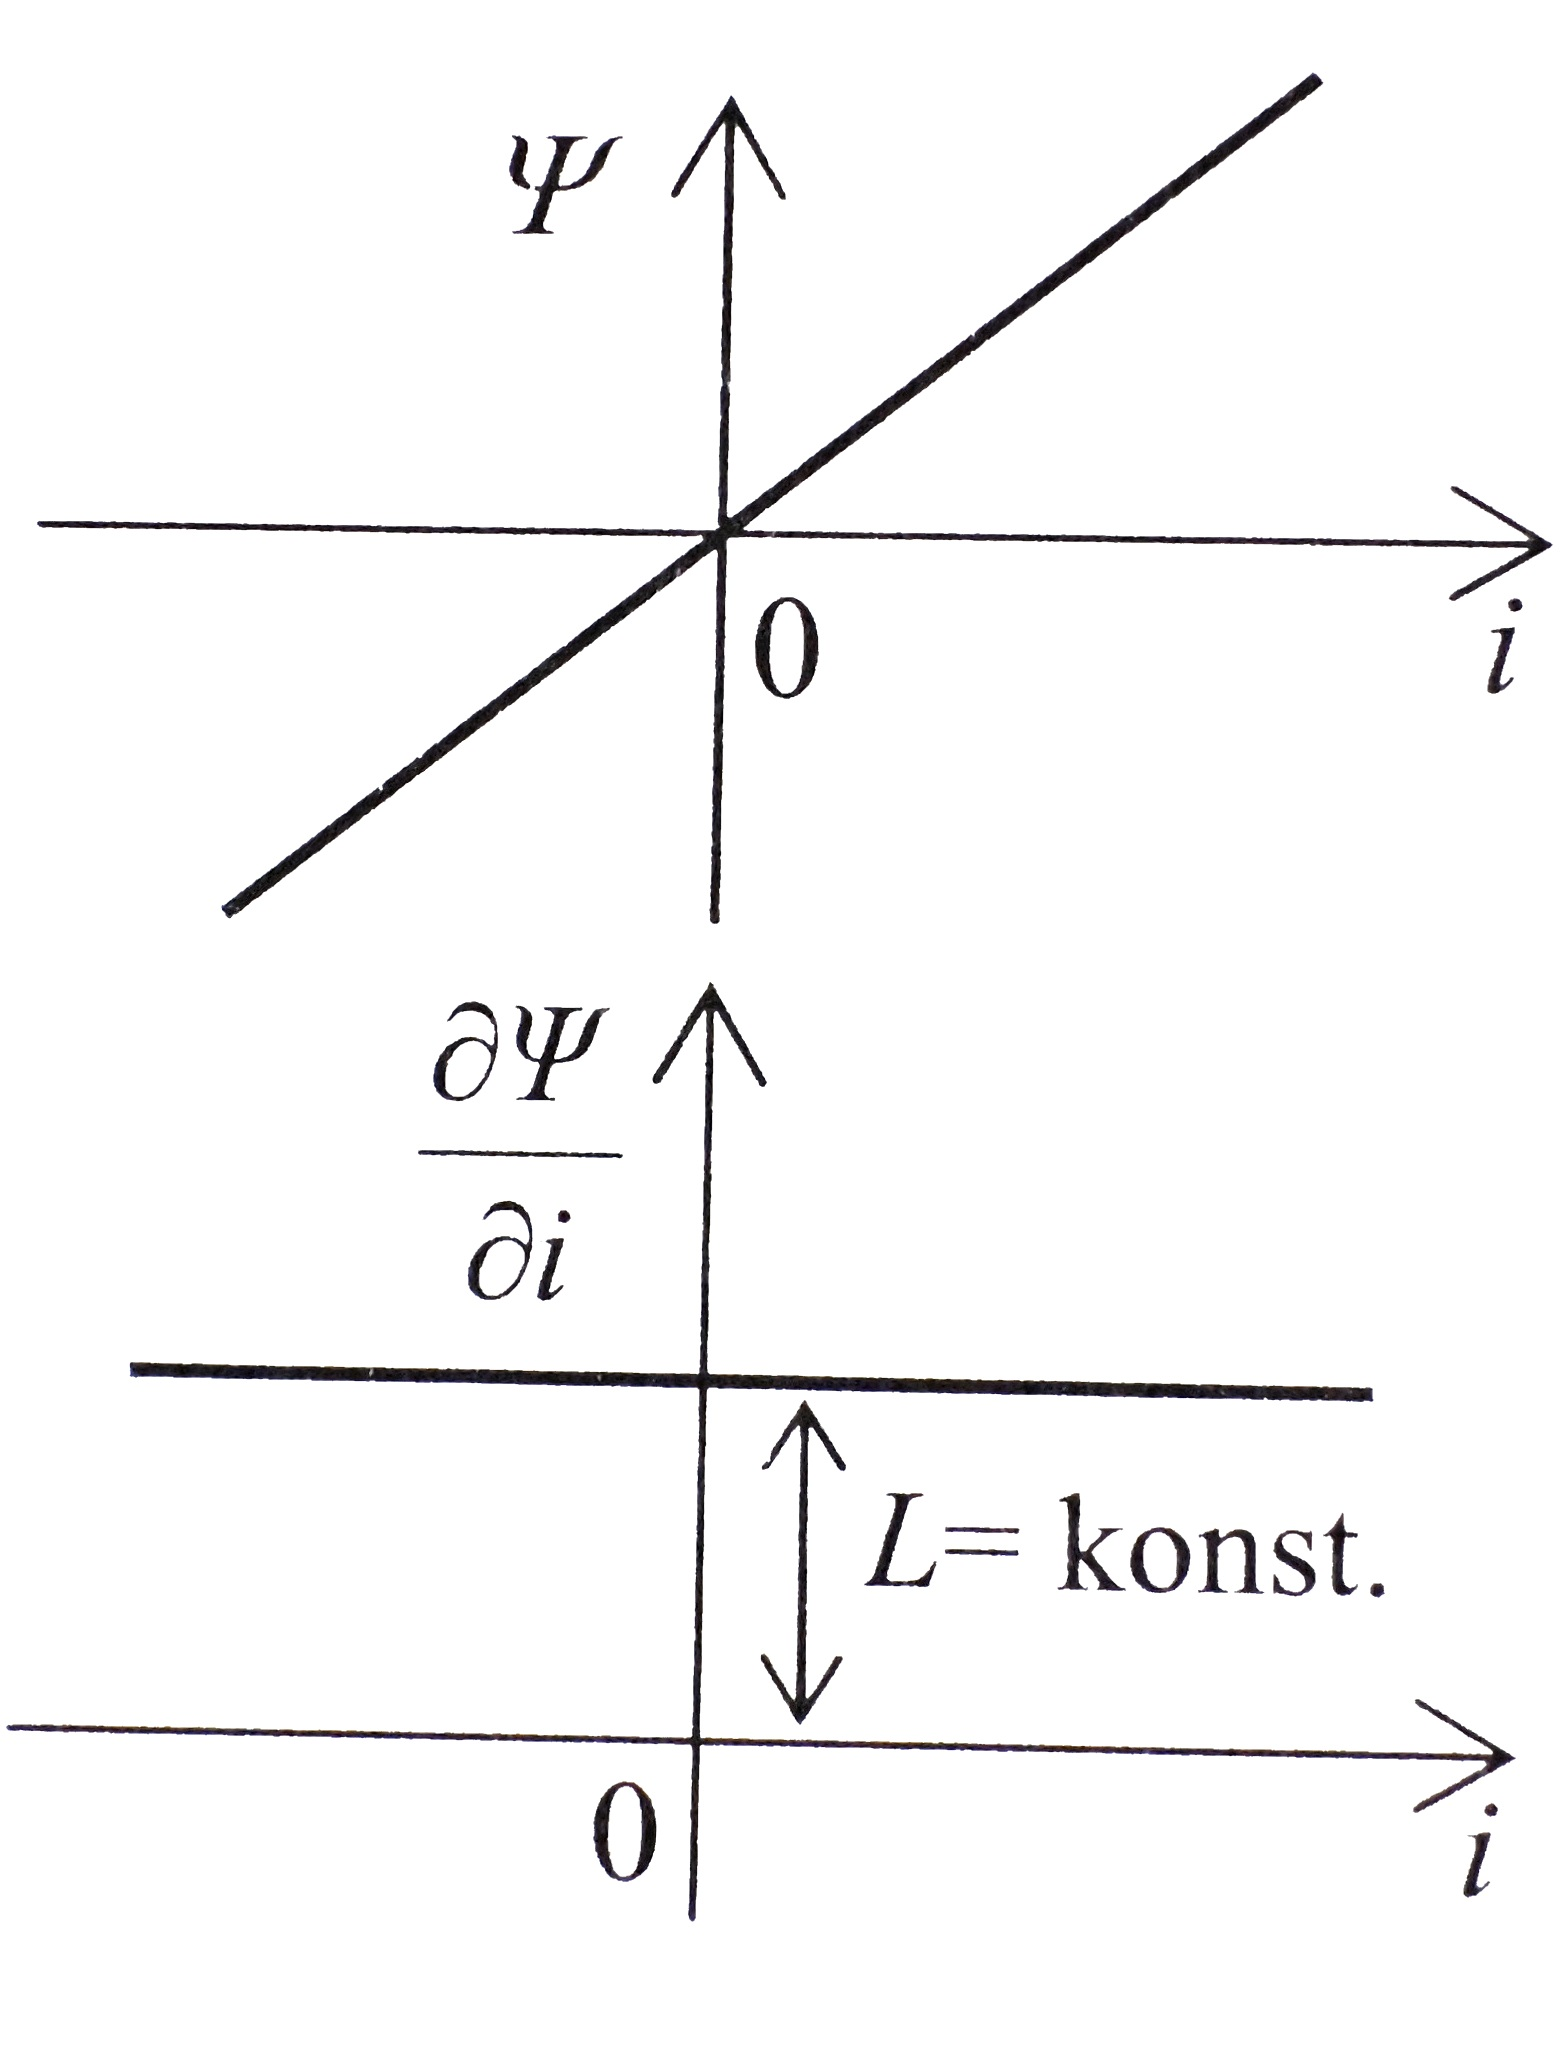
\includegraphics[width=0.4\linewidth]{teo_fig006.jpg}
        \caption{K výpočtu indukovaného napětí v lineárním magnetickém obvodu. Indukčnost má význam 
                 derivace toku podle proudu.
                (\cite[s.~154]{Patocka4})}
        \label{teo:fig006}
      \end{figure}
      Výpočet indukovaného napětí vychází z \emph{obecného} indukčního zákona, napsaného v 
      diferenciálním tvaru (\ref{vol02:TEO:eq108}), tj. z rovnice \(u(t) = \der{\Psi(t)}{t}\), do 
      které dosadíme pravou stranu rovnice (\ref{TEO:eq014}):
      \begin{equation}\label{TEO:eq016}
        \boxed{u(t) = \der{\Psi(t)}{t} = \der{Li(t)}{t} = L\der{i(t)}{t}}\,.
      \end{equation}
      Podstatný rozdíl mezi rovnicemi (\ref{vol02:TEO:eq108}) a (\ref{TEO:eq016}) spočívá v tom, 
      že první rovnice je platná \emph{obecně} v lineárních i nelineárních obvodech, kdežto druhá 
      platí pouze ve zvláštním případě \emph{lineárního magnetického obvodu}. Taktéž můžeme na 
      funkci (\ref{TEO:eq014}) formálně pohlížet jako na funkci složenou. Pak je její derivace 
      rovna součinu derivací vnější a vnitřní funkce:
      \begin{equation}\label{TEO:eq017}
        u(t) = \der{\Psi(t)}{t} = \underbrace{\pder{\Psi}{i}}_L\der{i(t)}{t} = L\der{i(t)}{t}
      \end{equation}
      Je vidět. že indukčnost má význam derivace toku podle proudu: \(L = \pder{\Psi}{i}\), což je 
      geometrický znázorněno na obr. \ref{teo:fig006}. Jedině u lineárního obvodu je tato derivace 
      \emph{konstantní} tj. nezávislá na proudu \(i\).
      
    \subsection{Energie lineárního magnetického obvodu}
      Diferenciální přírůstek magnetické energie lze vyjádřit pomocí \emph{okamžitého výkonu} 
      vztahem
      \begin{align}\label{TEO:eq018}
        dW(t) &= p(t)dt = u(t)\cdot i(t)dt                        \nonumber \\
              &= \der{\Psi}{t}i(t)dt = i(t)d\Psi(t).
      \end{align}
      Vidíme, že diferenciály času \(dt\) se vykrátily a zbyl pouze diferenciál toku \(d\Psi(t)\). 
      To znamená, že je nutno integrovat podle proměnné \(\Psi(t)\), resp. podle \(\Psi\), tak, jak 
      je naznačeno na obr. \ref{teo:fig007}. V geometrickém smyslu je tedy energie rovna ploše 
      ležící \textbf{nad} magnetizační charakteristikou, nikoli pod ní.
      
      \begin{figure}[ht!] %\ref{teo:fig007}
        \centering
        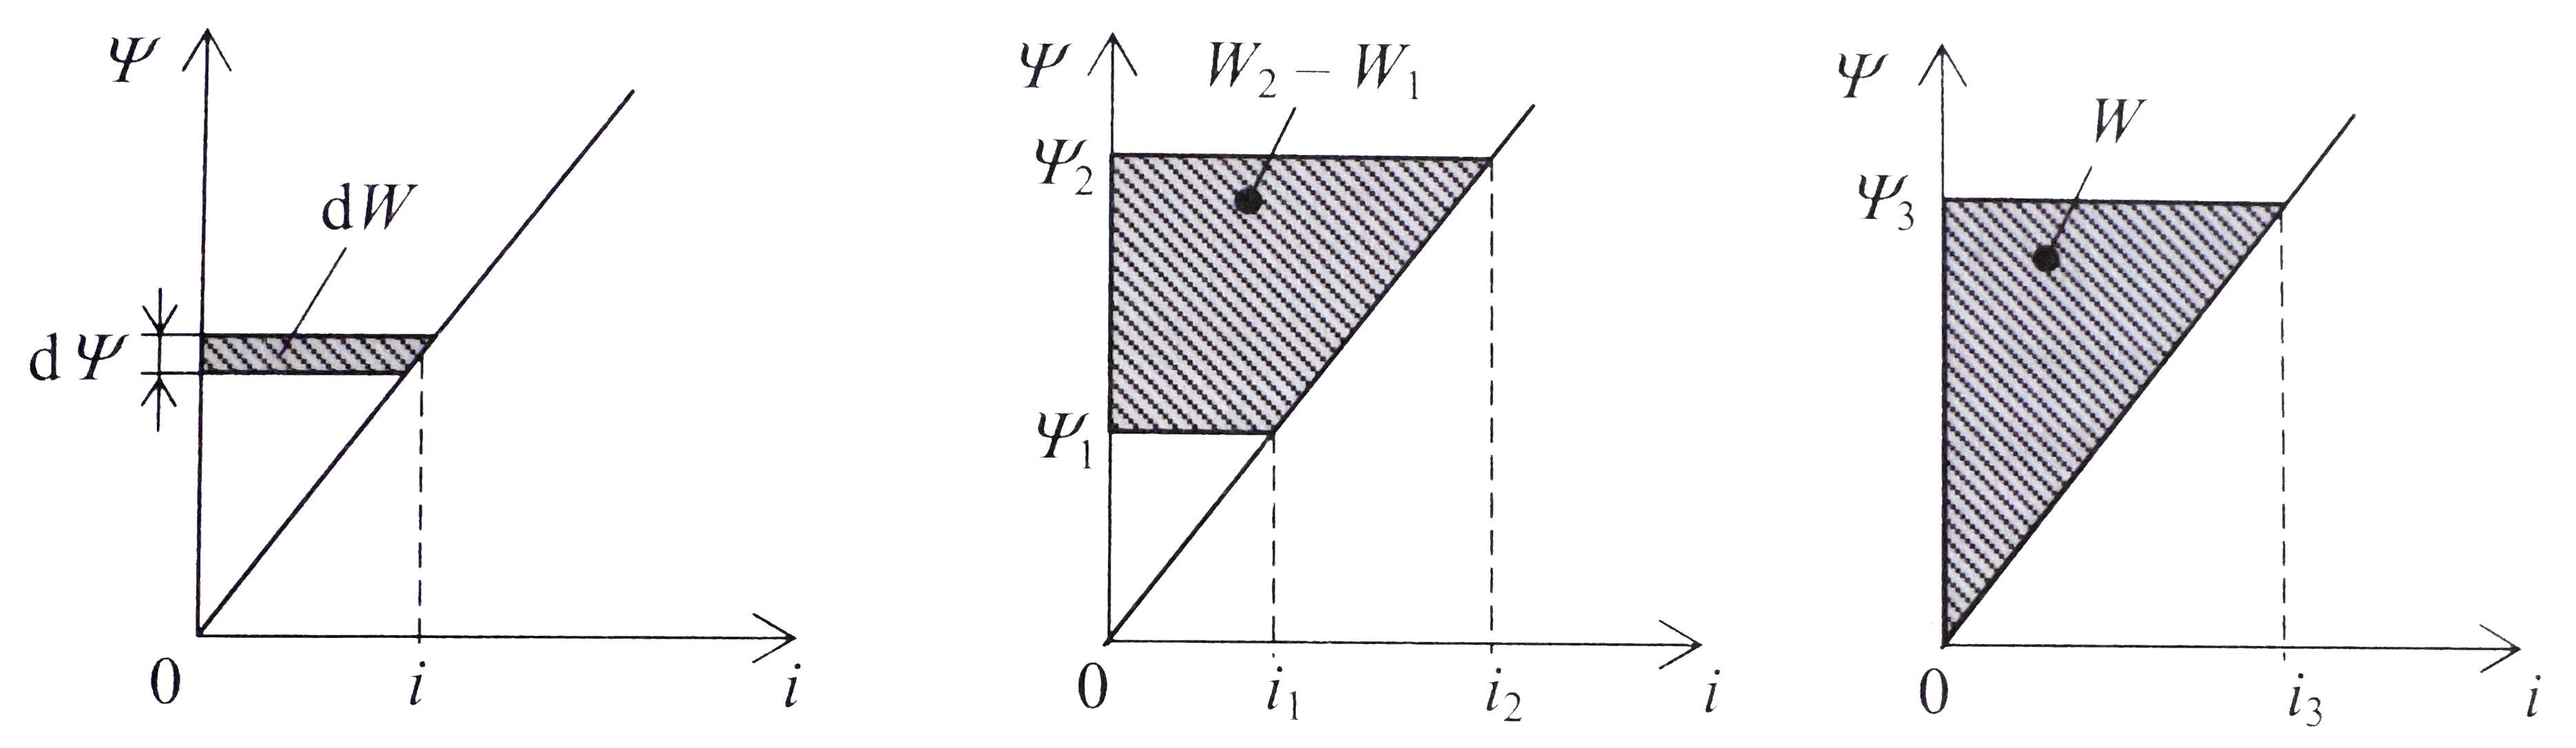
\includegraphics[width=0.99\linewidth]{teo_fig007.jpg}
        \caption{K výpočtu energie lineárního magnetického obvodu
                 (\cite[s.~155]{Patocka4})}
        \label{teo:fig007}
      \end{figure}
      Jedním ze způsobu jak vypočítat energii magnetického obvodu je dosazením pravé strany 
      inverzní magnetizační charakteristiky \ref{TEO:eq015} do rovnice \ref{TEO:eq018} za proud 
      \(i(t)\). 
      \begin{equation}\label{TEO:eq019}
        dW(t) = i(t)d\Psi(t) = \frac{\Psi(t)}{L}d\Psi(t).
      \end{equation}
      Integrací rovnice (\ref{TEO:eq019}) získáme okamžitou energii akumulovanou v magnetickém 
      obvodu
      \begin{align}\label{TEO:eq020}
        W(t) &= W_0 + \int_t\dd{W(t)}                            \nonumber \\ 
             &= W_0 + \int_{\Psi(t)}\frac{\Psi(t)}{L}\dd{W(t)} 
             = W_0 + \frac{1}{2}\frac{\Psi^2(t)}{L},
      \end{align}
      kde \(W_0\) je libovolná počáteční energie nashromážděná v cívce v předcházejícím ději. 
      Neurčitý integrál Lze přepsat na integrál určitý
      \begin{equation}\label{TEO:eq021}
        \boxed{W(t_2) - W(t_1)  = \frac{1}{2L}\left(\Psi^2(t_2) - \Psi^2(t_1)\right)}\,,
      \end{equation}
      který lze formálně přeznačit do \emph{statického} tvaru
      \begin{equation}\label{TEO:eq022}
        \boxed{W_2 - W_1 = \frac{1}{2L}(\Psi^2_2 - \Psi^2_1)}\,,
      \end{equation}
      
      Druhý způsob spočívá v dosazení pravé strany rovnice \ref{TEO:eq017} za napětí \(u(t)\) v 
      rovnici \ref{TEO:eq018}
      \begin{equation}\label{TEO:eq023}
        dW(t) = u(t)i(t)\dd{t} = L\der{i(t)}{t}i(t)\dd{t} = Li(t)\dd{i(t)}.
      \end{equation}
      Integrací rovnice (\ref{TEO:eq023}) získáme okamžitou energii akumulovanou v magnetickém obvod
      \begin{align}\label{TEO:eq024}
        W(t) &= W_0 + \int_t\dd{W(t)}                  \nonumber \\
             &= W_0 + L\int_{i(t)}i(t)\dd{i(t)} 
              = W_0 + \frac{1}{2}Li^2(t).
      \end{align}
      Neurčitý integrál lze přepsat na integrál určitý
      \begin{equation}\label{TEO:eq025}
        \boxed{W(t_2) - W(t_1)  = \frac{1}{2}L\left(i^2(t_2) - i^2(t_1)\right)}\,,
      \end{equation}
      který lze formálně přeznačit do \emph{statického} tvaru
      \begin{equation}\label{TEO:eq026}
        \boxed{W_2 - W_1 = \frac{1}{2}L(i^2_2 - i^2_1)}\,.
      \end{equation}
      Zdůrazněme, že všechny uvedené rovnice platí především \emph{dynamicky}, tj. v okamžitých 
      hodnotách. Známé statické tvary vyplynou z rovnic teprve sekundárně, jako zvláštní případy. 
      Je-li počáteční proud a tok nulový, pak lze zřejmě psát známé vztahy
      \begin{equation}\label{TEO:eq027}
        \boxed{W = \frac{1}{2}\frac{\Psi^2}{L} = \frac{1}{2}Li^2 = \frac{1}{2}\Psi i}\,.
      \end{equation}
      
  \section{Nelineární magnetický obvod}
    V této kapitole předpokládáme nelineární magnetizační charakteristiku bez hystereze, podle obr. 
    \ref{teo:fig008}. Matematické operace uvedené v této kapitole jsou nezbytné při realizaci 
    numerických matematických modelů nelineárních obvodů v prostředí Matlab-Simulink. Zde je možno 
    zadat nelineární magnetizační charakteristiku dvěma rozdílnými způsoby:
    \begin{itemize}
      \item Jako jednorozměrnou převodní tabulku \(B = B(H)\) nebo inverzní tabulku \(H = H(B)\),
            do nichž dosadíme dostatečně hustě skutečné naměřené hodnoty. Simulink sám automaticky
            dopočítá hodnoty mezí sousedními body pomocí polynomů a vytvoří tak plynulou funkci.
      \item Jako analytickou funkci (\ref{TEO:eq011}), odvozenou v příslušné kapitole z vnitřních
            fyzikálních dějů ve feromagnetiku.
    \end{itemize}
    Pokud je magnetický obvod bez vzduchové mezery, magnetizační charakteristiku \(\Psi = \Psi(i)\) 
    lze získat z přímce \(B = B(H)\) pomocí známých převodních vztahů:
    \begin{equation}  \label{TEO:eq012}
      \Psi(t) \cong N\Phi = NS_{Fe}B(H), \qquad i = \dfrac{l_{Fe}}{N}H.
    \end{equation}
    
    \subsection{Výpočet indukovaného napětí}
      Magnetizační charakteristika nelineárního magnetického obvodu má tvar obecné nelineární 
      funkce 
      \begin{equation}\label{TEO:eq028}
        \Psi    = \Psi[i], \quad\text{resp.}\quad
        \Psi(t) = \Psi[i(t)].
      \end{equation}
      Z formálního matematického pohledu lze na magnetizační charakteristiku \(\Psi = \Psi[i]\) 
      pohlížet jako na \emph{složenou} funkci dynamickou \(\Psi(t) = \Psi[i(t)]\), kde hranatými 
      závorkami je vyznačena \emph{vnější} statická funkce proudu a závorkami kulatými je vyznačena 
      \emph{vnitřní} dynamická funkce času. Z rovnic (\ref{TEO:eq028}) lze získat inverzní 
      magnetizační charakteristiku:
      \begin{equation}\label{TEO:eq029}
        i = i[\Psi], \qquad\text{resp.}\qquad i(t) = i[\Psi(t)].
      \end{equation}

      \begin{figure}[ht!]  %\ref{teo:fig008}
        \centering
        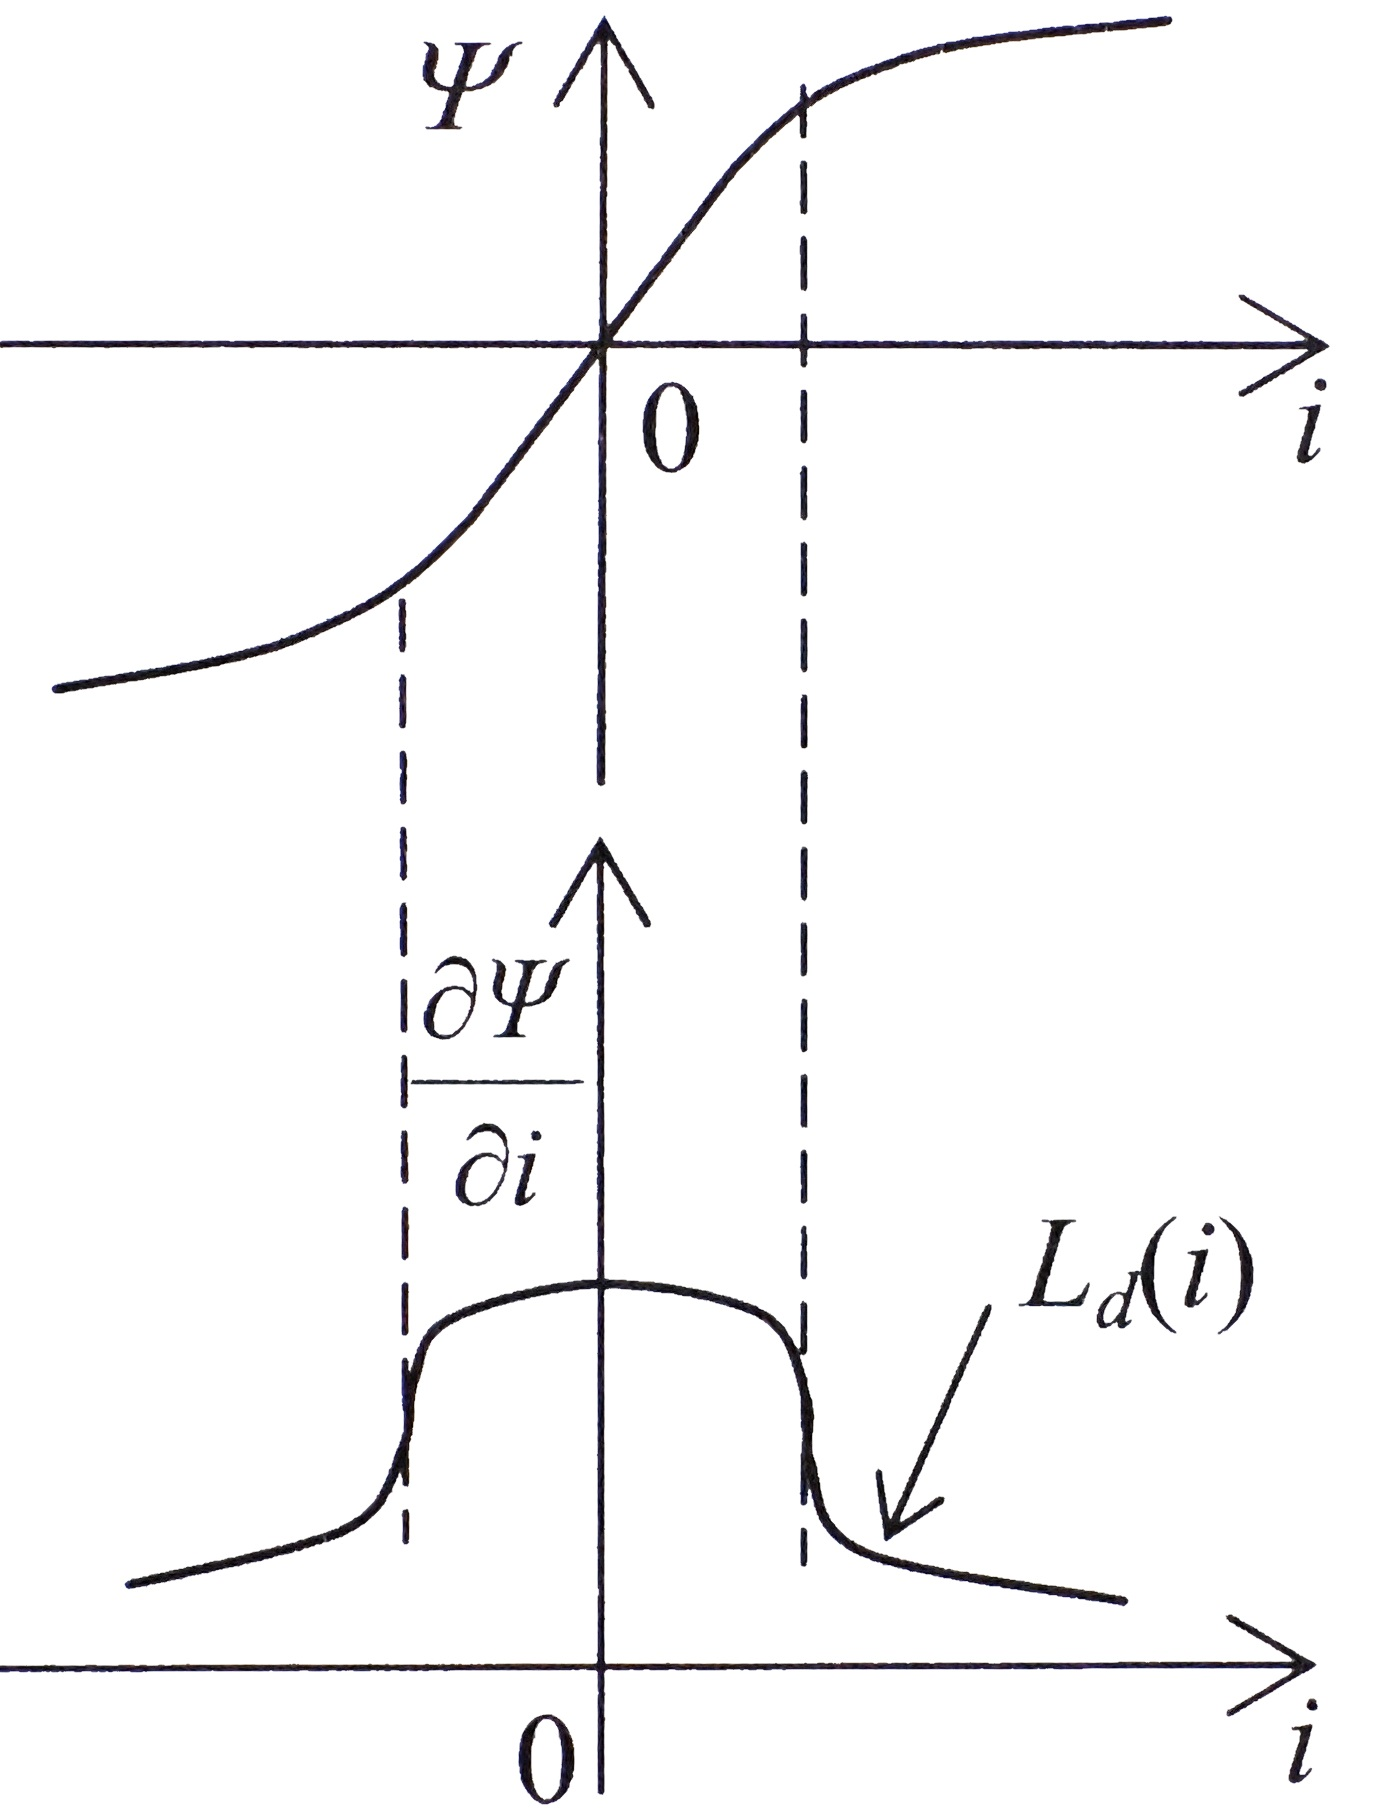
\includegraphics[width=0.5\linewidth]{teo_fig008.jpg}
        \caption{K výpočtu indukovaného napětí v nelineárním magnetickém obvodu. 
                (\cite[s.~157]{Patocka4})}
        \label{teo:fig008}
      \end{figure}
      
      Výpočet indukovaného napětí vychází z \emph{obecného} indukčního zákona napsaného v 
      diferenciálním tvaru (\ref{vol02:TEO:eq108}), tj. z rovnice \(u(t) = \der{\Psi(t)}{t}\), do 
      které dosadíme složenou funkci (\ref{TEO:eq028}). Pak je její derivace rovna součinu derivací 
      vnější a vnitřní funkce:
      \begin{align}\label{TEO:eq030}
        u(t) &= \der{\Psi(t)}{t} = \der{\Psi[i(t)]}{t}                \nonumber \\
             &= \underbrace{\pder{\Psi[i]}{i}}_{L_d[i]}\der{i(t)}{t} 
              = L_d[i]\der{i(t)}{t}\,.
      \end{align}
      
      Je vidět, že význam má pouze \textbf{diferenciální indukčnost}, tj. \emph{směrnice tečny k 
      magnetizační charakteristice}, což je geometricky znázorněno na obr. \ref{teo:fig008}. 
      Zdůrazněme, že indukčnost počítaná jako směrnice sečny nemá ani matematický ani fyzikální 
      význam. Proto je v matematických modelech nutno pracovat s \emph{diferenciální 
      permeabilitou}, nikoli s \emph{permeabilitou amplitudovou}.
      
      Z obr. \ref{teo:fig008} plyne, že diferenciální indukčnost \(L_d\) je přibližně konstantní v 
      nepřesycené oblasti magnetizační charakteristiky. Vně této oblasti indukčnost rychle klesá, 
      při velikých proudech až na indukčnost samotné vzduchové cívky (jako bychom z cívky 
      odstranili feromagnetické jádro).
      
    \subsection{Energie nelineárního magnetického obvodu}
      Postup výpočtu je stejný jako u lineárního obvodu. Diferenciální přírůstek magnetické energie 
      je nutno vyjádřit rovněž pomocí \emph{okamžitého výkonu} vztahem
      \begin{align}\label{TEO:eq031}
        dW(t) &= p(t)\dd{t} = u(t)\cdot i(t)\dd{t}         \nonumber \\
              &= i(t)\dd{t}\der{\Psi}{t} = i(t)d\Psi(t).
      \end{align}

      \begin{figure}[ht!] %\ref{teo:fig009}
        \centering
        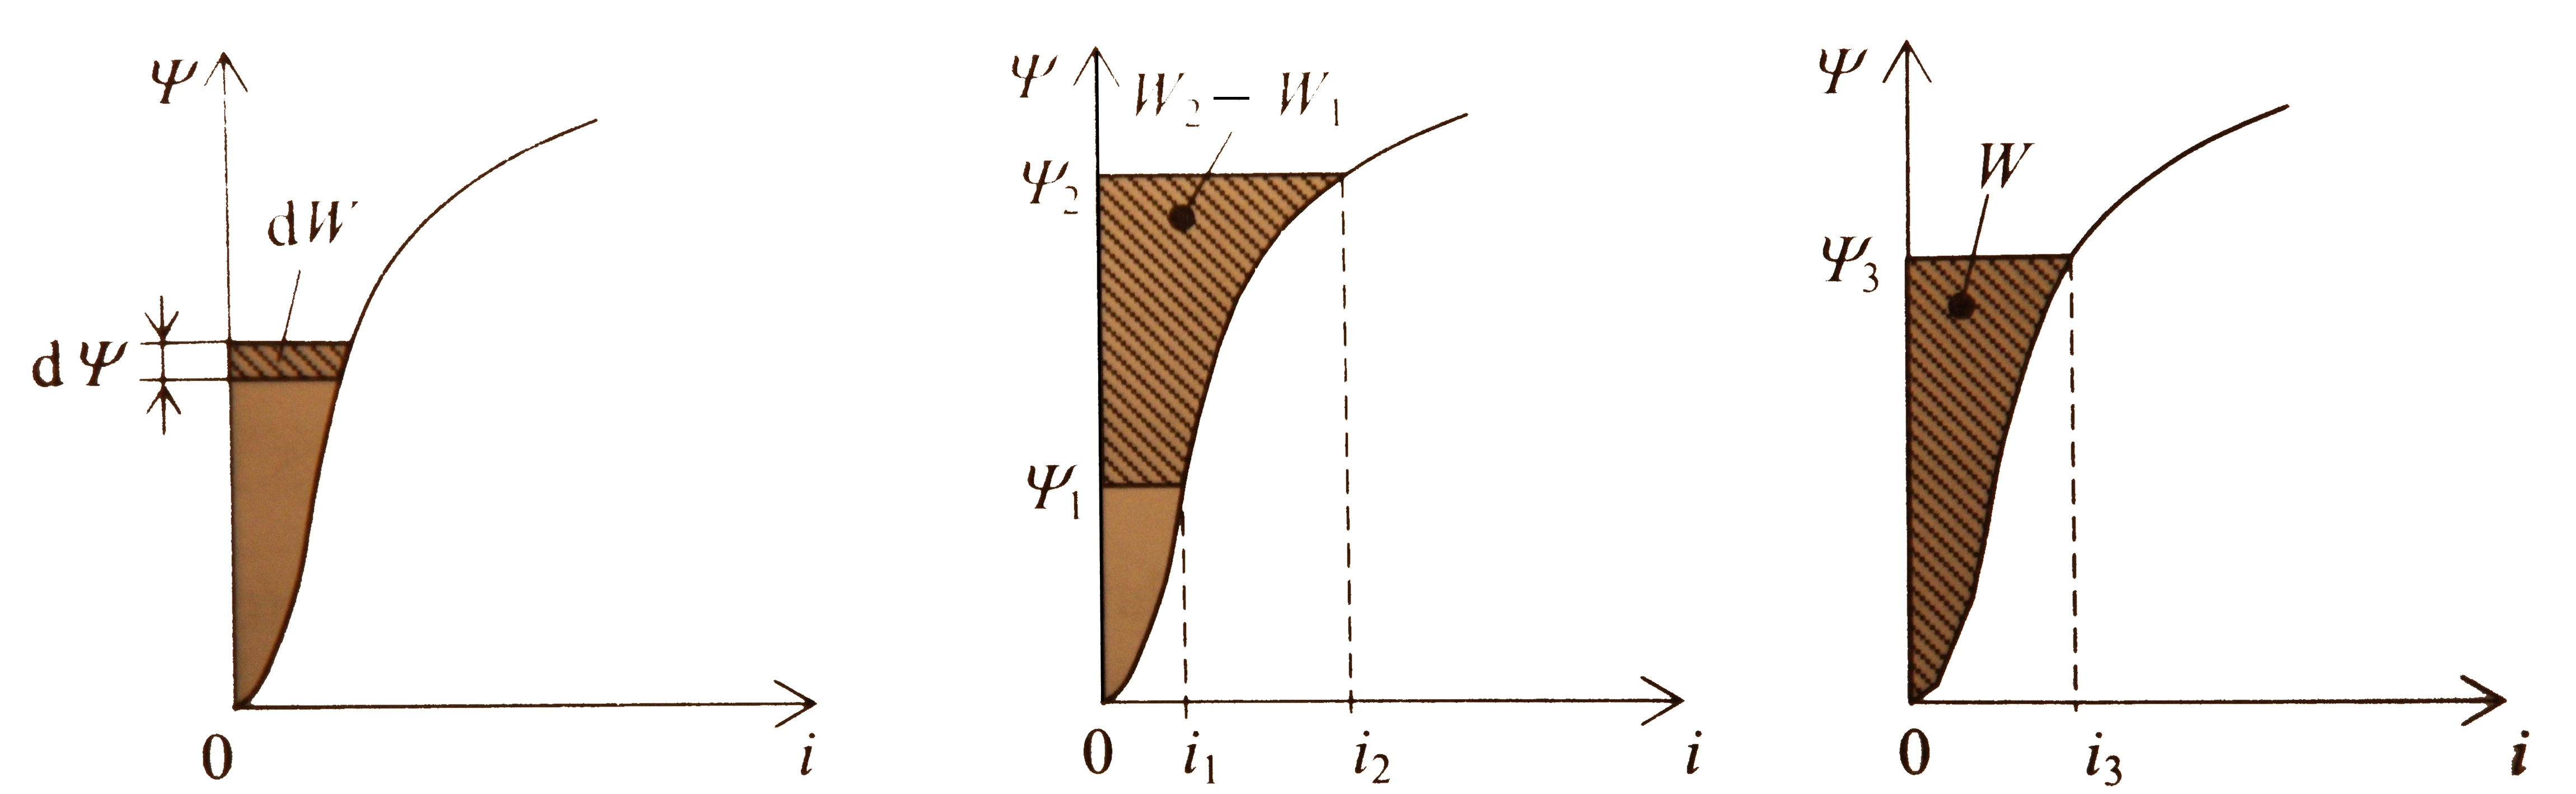
\includegraphics[width=0.99\linewidth]{teo_fig009.jpg}
        \caption{K výpočtu energie nelineárního magnetického obvodu
                 (\cite[s.~158]{Patocka4})}
        \label{teo:fig009}
      \end{figure}
      Diferenciály času \(\dd{t}\) v rovnici (\ref{TEO:eq031}) se vykrátily a zbyl pouze 
      diferenciál toku \(\dd{\Psi(t)}\). To znamená, že je nutno integrovat podle proměnné 
      \(\Psi(t)\), tak, jak je naznačenou na obr. \ref{teo:fig009}. V geometrickém smyslu je tedy 
      energie rovna ploše ležící nad magnetizační charakteristikou, nikoli pod ní.

      První způsob výpočtu energii magnetického obvodu je dosazením pravé strany 
      inverzní magnetizační charakteristiky \ref{TEO:eq029} do rovnice \ref{TEO:eq031} za proud 
      \(i(t)\). 
      \begin{equation}\label{TEO:eq032}
        dW(t) = i(t)\dd{\Psi(t)} = i[\Psi(t)]\dd{\Psi(t)}.
      \end{equation}
      Integrací rovnice (\ref{TEO:eq032}) získáme okamžitou energii akumulovanou v magnetickém 
      obvodu
      \begin{equation}\label{TEO:eq033}
        W(t) = W_0 + \int_t\dd{W(t)} = W_0 + \int_{\Psi(t)}i[\Psi(t)]\dd{\Psi(t)},
      \end{equation}
      kde \(W_0\) je libovolná počáteční energie nashromážděná v cívce v předcházejícím ději. 
      Neurčitý integrál Lze přepsat na integrál určitý
      \begin{equation}\label{TEO:eq034}
        \boxed{W(t_2) - W(t_1)  = \int_{\Psi(t_1)}^{\Psi(t_2)}i[\Psi(t)]\dd{\Psi(t)}}\,,
      \end{equation}
      který lze formálně přeznačit do \emph{statického} tvaru
      \begin{equation}\label{TEO:eq035}
        \boxed{W_2 - W_1  = \int_{\Psi_1}^{\Psi_2}i[\Psi]\dd{\Psi}}\,,
      \end{equation}
      
      Druhý způsob spočívá v dosazení pravé strany rovnice \ref{TEO:eq030} za napětí \(u(t)\) v 
      rovnici \ref{TEO:eq031}
      \begin{align}\label{TEO:eq036}
        dW(t) &= u(t)i(t)\dd{t}                            \nonumber \\
              &= L_d[i]\der{i(t)}{t}i(t)\dd{t} = L_d[i]i(t)\dd{i(t)}.
      \end{align}
      Integrací rovnice (\ref{TEO:eq036}) získáme okamžitou energii akumulovanou v magnetickém obvod
      \begin{equation}\label{TEO:eq037}
        W(t) = W_0 + \int_t\dd{W(t)} = W_0 + \int_{i(t)} L_d[i]i(t)\dd{i(t)}.
      \end{equation}
      Neurčitý integrál lze přepsat na integrál určitý
      \begin{equation}\label{TEO:eq038}
        \boxed{W(t_2) - W(t_1)  = \int_{i(t_1)}^{i(t_2)} L_d[i]i(t)\dd{i(t)}}\,,
      \end{equation}
      který lze formálně přeznačit do \emph{statického} tvaru
      \begin{equation}\label{TEO:eq039}
        \boxed{W_2 - W_1 = \int_{i_1}^{i_2} L_d[i]i\dd{i}}\,,
      \end{equation}
      Zdůrazněme, že všechny uvedené rovnice platí především \emph{dynamicky}, tj. v okamžitých 
      hodnotách. Známé statické tvary vyplynou z rovnic teprve sekundárně, jako zvláštní případy. 
      
    \subsection{Hysterezní ztráty}
      Ztrátová energie, přeměněná v teplo při jednom oběhu hysterezní smyčky, je přímo rovna ploše 
      smyčky podle Obr. \ref{teo:fig010}. Tvrzení jasně plyne z výpočtu provedených v předchozí 
      kapitole. Porovnáme-li obr. \ref{teo:fig010} s obr. \ref{teo:fig009}, pak vidíme, že energie 
      \(W_{1,2}\) akumulovaná v magnetickém obvodu při pohybu z bodu \(1\) do \(2\) je větší než 
      energie \(W_{2,1}\) odevzdaná zpět do zdroje při pohybu z bodu \(2\) do \(1\). Rozdíl obou 
      energií je pak roven tepelné ztrátové hysterezní energii \(W_H\), která má velikost
      \begin{equation}\label{TEO:eq040}
        W_H = W_{1,2} - W_{2,1}\,.
      \end{equation}
      Rovnice souhlasí rozměrově, neboť \([J] = [W\cdot s] = [Wb]\cdot[A] = [V\cdot s]\cdot[A]\).
      
      \begin{figure}[ht!] %\ref{teo:fig010}
        \centering
        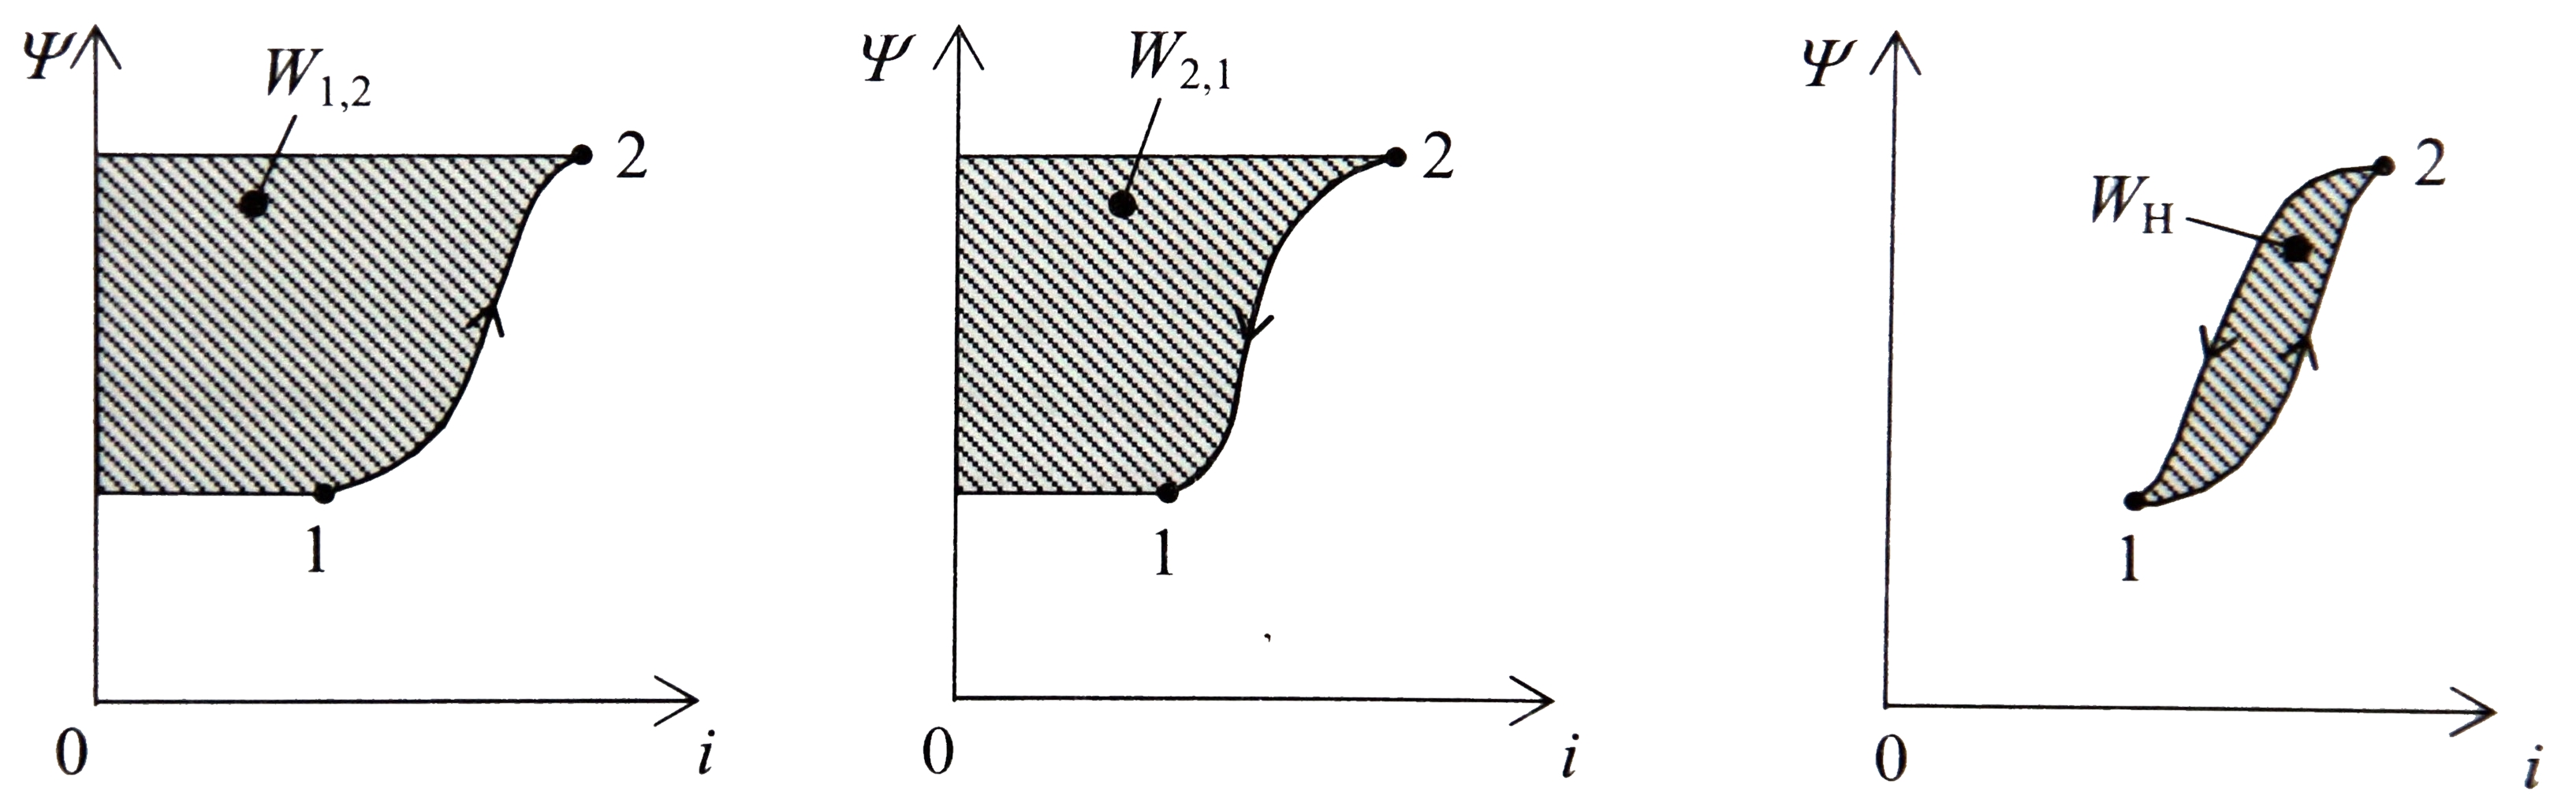
\includegraphics[width=0.99\linewidth]{teo_fig010.jpg}
        \caption{K výpočtu ztrátové energie hysterezní smyčky.
                 (\cite[s.~159]{Patocka4})}
        \label{teo:fig010}
      \end{figure}
      
      Pokud pracujeme s normovanou magnetizační charakteristikou \(B = B(H)\), pak má plocha 
      \(S_H\) hysterezní smyčky význam \textbf{měrné ztrátově energie} vztažené na \(\SI{1}{m^3}\) 
      neboť rozměrově lze psát
      \begin{equation*}
        \left[\frac{J}{m^3}\right] = [T]\left[\frac{A}{m}\right] 
                                   = \left[\frac{V\cdot s}{m^2}\right]\left[\frac{A}{m}\right] \,.
      \end{equation*}
      \emph{Ztrátový hysterezní Činný výkon} - jako každý \emph{činný} výkon - musí být definován 
      jako \emph{střední hodnota okamžitého výkonu} na opakovači periodě \(T\): 
      \begin{align}\label{TEO:eq041}
        P_H &= \frac{1}{T}\int_0^Tp(t)\dd{t}          \nonumber \\
            &= \frac{1}{T}W_H = fS_HV_{Fe}
               \qquad[W;Hz, J/m^3, m^3]\,.
      \end{align}
      Objem feromagnetika \(V_{Fe}\) lze pomocí měrné hmotnosti \(\gamma_{Fe}\) přepočítat na 
      hmotnost \(m_{Fe}\): 
      \begin{align}\label{TEO:eq042}
        P_H &= fS_HV_{Fe}                            \nonumber \\
            &= f\frac{S_H}{\gamma_{Fe}}m_{Fe} = Zm_{Fe} 
               \qquad[W; W/kg, kg]\,,
      \end{align}
      kde \(Z\) má význam \emph{ztrátového čísla}, tj. \textbf{měrných ztrát}. V praxi by bylo 
      nutno započíst do měrných ztrát i ztráty vířivé, které byly odvozeny v kapitole 
      \ref{teo:IchapIVsecI}.
      
  \section{Nelineární parametrický magnetický obvod}
    V této kapitole předpokládáme nelineární magnetizační charakteristiku závislou na libovolném 
    parametru \(p\), podle obr. \ref{teo:fig001e}. Kapitola se týká všech typů reluktančních strojů:
    \begin{itemize}
      \item  \emph{Levitační elektromagnet} - parametrem \(p\) je proměnná délka \(l\) vzduchové 
             mezery.
      \item \emph{Parametrický bezdotykový snímač vzdálenosti} - parametrem \(p\) je proměnná délka 
            vzduchové mezery.
      \item \emph{Spínaný reluktanční motor} - parametrem \(p\) je proměnná šířka \(S_{Fe}\) 
            vzduchové mezery, vymezená překrývajícími se pólovými nástavci statoru a pohyblivého 
            rotoru.
      \item \emph{Pracovní tažný elektromagnet} - parametrem \(p\) je proměnná plocha \(S_{Fe}\)    
            magnetického obvodu, vymezená překrývajícími se pólovými nástavci pevné a posuvné části.
    \end{itemize}
    
    Matematické operace uvedené v této kapitole jsou nezbytné při realizaci numerických 
    matematických modelů všech zmíněných reluktančních strojů v prostředí \texttt{Matlab - 
    Simulink}. Zde je možno zadávat změřenou nelineární magnetizační charakteristiku jako 
    dvojrozměrnou převodní tabulku \(B = B(H,p)\), nebo inverzní \emph{dvojrozměrnou} tabulku \(H = 
    H(B, p)\). Obsahuje-li magnetický obvod vzduchovou mezeru \(l\), pak platí rovnice
    \begin{equation}\label{TEO:eq043}
      Ni = H_0l + Hl_{Fe} = \frac{B(H)}{\mu_0}l + Hl_{Fe}.
    \end{equation}
    V takovém případe 1ze získat charakteristiku \(\Psi = \Psi[i,p]\) z původní magnetizační 
    charakteristiky \(B=B(H)\) samotného feromagnetického materiálu pomocí převodních vztahů

    \begin{align}
      \Psi &\cong N\Phi = NS_{Fe}B(H),                       \label{TEO:eq044} \\
         i &= \frac{B(H)}{N\mu_0}l + \frac{l_{Fe}}{N}H.      \label{TEO:eq045}
    \end{align} 
    Vztah (\ref{TEO:eq045}) vznikl úpravou rovnice (\ref{TEO:eq043}). Podle typu reluktančního 
    stroje je nutno v rovnicích (\ref{TEO:eq044}), (\ref{TEO:eq045}) považovat za parametr buď 
    proměnlivou plochu \(S_{Fe}\) nebo proměnlivou délku vzduchové mezery \(l\). Poznamenejme, že 
    parametrem může být samozřejmě v obecnějším smyslu i jakákoli jiná fyzikální veličina (teplota, 
    tlak...).

    \subsection{Výpočet indukovaného napětí}
      Magnetizační charakteristika nelineárního magnetického obvodu má tvar obecné nelineární funkce
      \begin{align}\label{TEO:eq046}
        \Psi    &= \Psi[i,p], \quad\text{resp.}   \nonumber \\
        \Psi(t) &= \Psi[i(t), p(t)].
      \end{align}
    
      Z matematického pohledu lze na magnetizační charakteristiku \(\Psi = \Psi[i,p]\) pohlížet 
      jako na složenou funkci dynamickou \(\Psi(t) = \Psi[i(t),p(t)]\), kde hranatými závorkami je 
      vyznačena \emph{vnější} statická funkce proudu a závorkami kulatými jsou vyznačeny obě 
      \emph{vnitřní} dynamické funkce času. Z rovnic (\ref{TEO:eq046}) lze získat inverzní 
      magnetizační charakteristiku ve tvaru
      \begin{equation}\label{TEO:eq047}
        i = i[\Psi, p], \quad\text{resp.}\quad i(t) = i[\Psi(t), p(t)].
      \end{equation}

      \begin{figure}[ht!]  %\ref{teo:fig011}
        \centering
        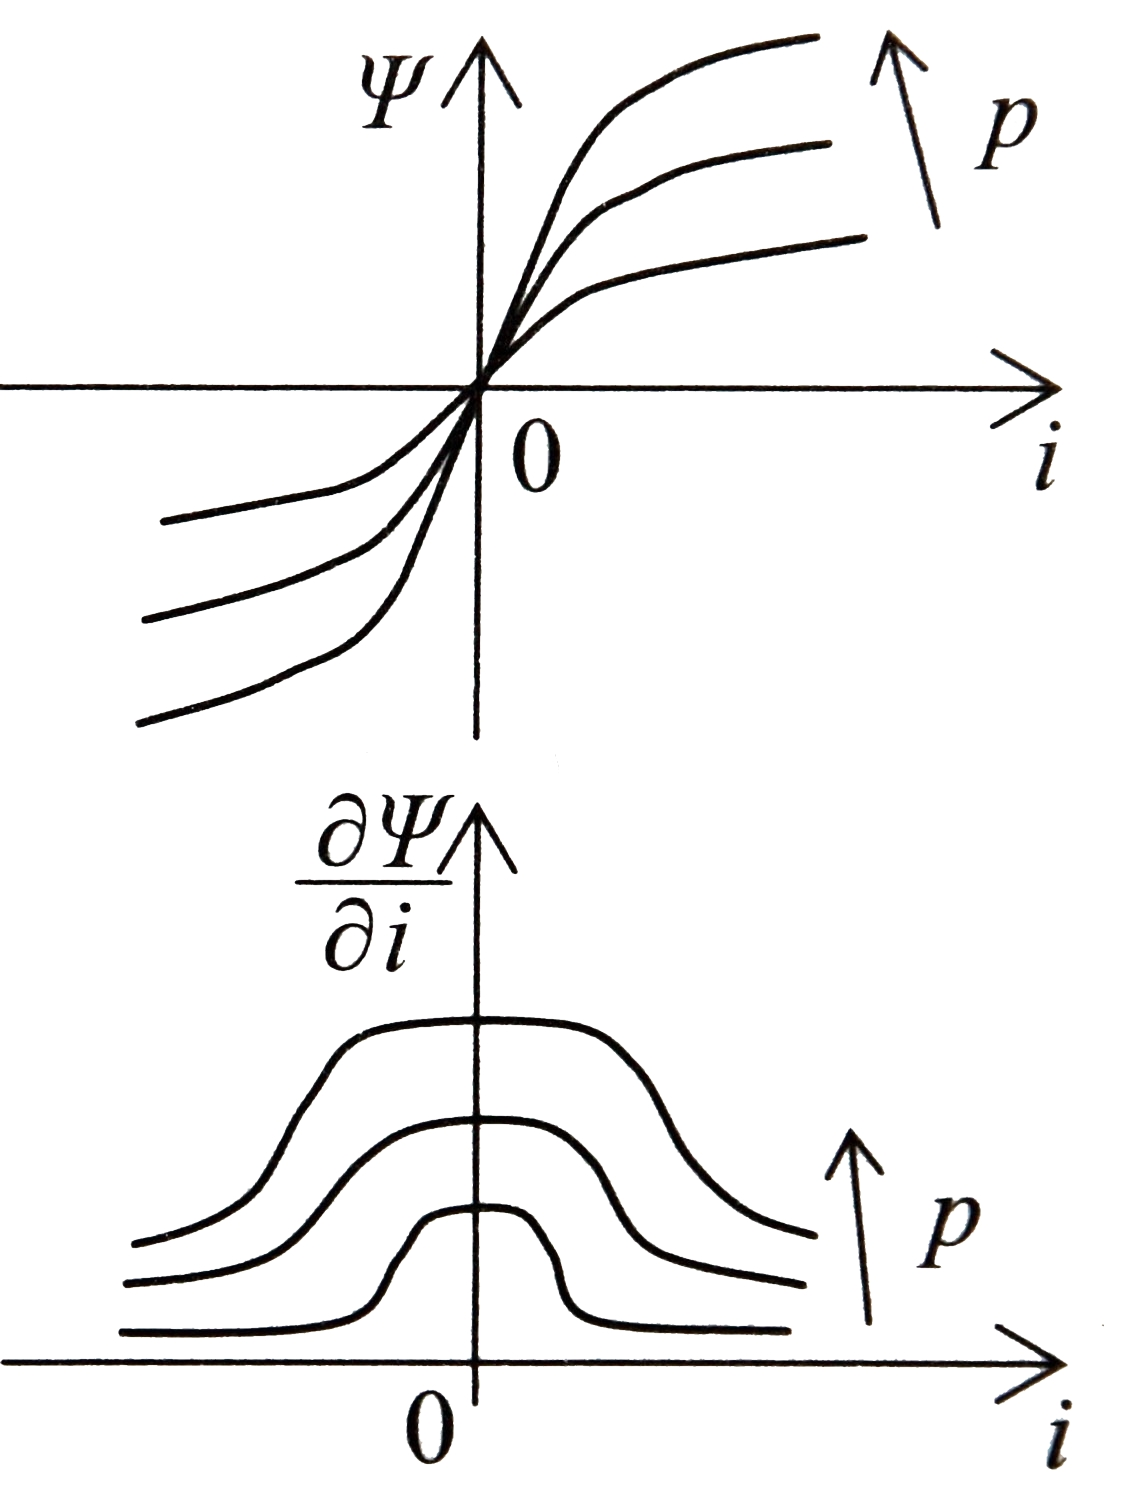
\includegraphics[width=0.5\linewidth]{teo_fig011.jpg}
        \caption{K výpočtu indukovaného napětí v nelineárním parametrickém magnetickém obvodu. 
                (\cite[s.~161]{Patocka4})}
        \label{teo:fig011}
      \end{figure}
      
      Výpočet indukovaného napětí vychází z \emph{obecného} indukčního zákona napsaného v 
      diferenciálním tvaru (\ref{vol02:TEO:eq108}), tj. z rovnice \(u(t) = \der{\Psi(t)}{t}\), do 
      které dosadíme složenou funkci (\ref{TEO:eq046}):
      \begin{align}
        u(t) &= \der{\Psi(t)}{t} = \der{\Psi[i(t),p(t)]}{t}                   \nonumber \\
             &= \pder{\Psi[i, p]}{i}\der{i(t)}{t} 
              + \pder{\Psi[i, p]}{p}\der{p(t)}{t}                             \nonumber \\
             &= L_d[i,p]\der{i(t)}{t} 
              + K_v[i,p]\der{i(t)}{t}\,.                                      \label{TEO:eq048}
      \end{align}
      kde 
           
      \noindent\begin{tabularx}{\linewidth}{@{}XX@{}}
        \begin{equation}\label{TEO:eq049}
           L_d[i,p]=\pder{\Psi[i, p]}{i},
        \end{equation} & 
        \begin{equation}\label{TEO:eq050}
           K_v[i,p] = \pder{\Psi[i, p]}{p}.
        \end{equation} 
      \end{tabularx}
      
      Diferenciální indukčnost \(L_d\) má význam \emph{směrnice tečny} k magnetizační 
      charakteristice, což je geometricky znázorněno na obr. \ref{teo:fig011}. Rychlostní funkce 
      \(K_v\) tvoří převod mezi rychlosti \(\der{p(t)}{t}\), s jakou se mění parametr \(p\) v 
      čase, a mezi \emph{rychlostní složkou} indukovaného napětí.

      % --------example: Levitační elektromagnet  ------------
      % \label{TEO:exam005}
      % !TeX spellcheck = cs_CZ
\begin{example}
  \textbf{Levitační elektromagnet}: Určeme indukované napětí na svorkách cívky levitačního 
  elektromagnetu podle obr \ref{teo:fig012}.
  
   {\centering
    \captionsetup{type=figure}
    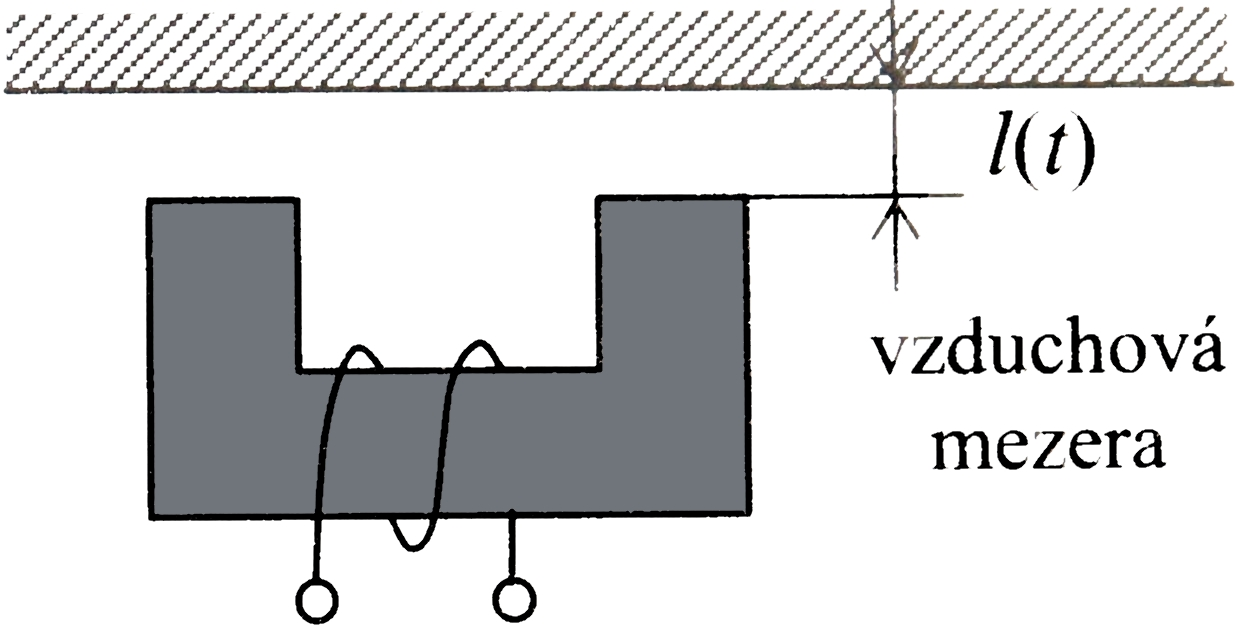
\includegraphics[width=0.6\linewidth]{teo_fig012.jpg}
    \captionof{figure}{Levitační elektromagnet jako příklad nelineárního parametrického 
               magnetického obvodu. (\cite[s.~161]{Patocka4})}
    \label{teo:fig012}
  \par}
  Z obrázku je zřejmé, že parametrem \(p(t)\) je délka \(l(t)\) vzduchové mezery. Tuto délku 
  dosadíme do rovnice (\ref{TEO:eq048}) namísto \( p(t)\):
  \begin{align}\label{TEO:eq076}
    u(t) &= \pder{\Psi[i, l]}{i}\der{i(t)}{t} + \pder{\Psi[i,l]}{l}\der{l(t)}{t}  \nonumber \\
         &= L_d[i,l]\der{i(t)}{t} + K_v[i,l]v(t)\,.
  \end{align}
  Indukované napětí levitačního elektromagnetu obsahuje dvě složky: první je úměrná derivaci proudu 
  a odpovídá napětí na diferenciální indukčnosti, druhá je úměrná vertikální rychlostí jha (tato 
  složka vzniká při pohybu i v případě, že proud cívkou udržujeme na \emph{konstantní} hodnotě!

\end{example}


  
      %-------------------------------------------------------
      
    \subsection{Energie nelineárního parametrického magnetického obvodu}
     Postup výpočtu je stejný jako u obvodu lineárního. Diferenciální přírůstek magnetické energie 
     je nutno vyjádřit rovněž pomocí \emph{okamžitého výkonu} vztahem
      \begin{align}\label{TEO:eq051}
        dW(t) &= p(t)\dd{t} = u(t)\cdot i(t)\dd{t}     \nonumber \\
              &= i(t)\dd{t}\der{\Psi}{t} = i(t)d\Psi(t).
      \end{align}
      Diferenciály času \(\dd{t}\) v rovnici (\ref{TEO:eq051}) se vykrátily a zbyl pouze 
      diferenciál toku \(\dd{\Psi(t)}\). To znamená, že je nutno integrovat podle proměnné 
      \(\Psi(t)\), tak, jak je naznačenou na obr. \ref{teo:fig009}. V geometrickém smyslu je tedy 
      energie rovna ploše ležící \emph{nad} magnetizační charakteristikou, nikoli pod ní.
      
      První způsob výpočtu energii magnetického obvodu je dosazením pravé strany 
      inverzní magnetizační charakteristiky \ref{TEO:eq047} do rovnice \ref{TEO:eq051} za proud 
      \(i(t)\). 
      \begin{equation}\label{TEO:eq052}
        dW(t) = i(t)\dd{\Psi(t)} = i[\Psi(t), p(t)]\dd{\Psi(t)}.
      \end{equation}
      Integrací rovnice (\ref{TEO:eq052}) získáme okamžitou energii akumulovanou v magnetickém 
      obvodu
      \begin{align}\label{TEO:eq053}
        W(t) &= W_0 + \int_t\dd{W(t)}                              \nonumber \\
             &= W_0 + \int_{\Psi(t)}i[\Psi(t), p(t)]\dd{\Psi(t)},
      \end{align}
      kde \(W_0\) je libovolná počáteční energie nashromážděná v cívce v předcházejícím ději. 
      Neurčitý integrál Lze přepsat na integrál určitý
      \begin{equation}\label{TEO:eq054}
        \boxed{W(t_2) - W(t_1)  = \int_{\Psi(t_1)}^{\Psi(t_2)}i[\Psi(t), p(t)]\dd{\Psi(t)}}\,,
      \end{equation}
      který lze formálně přeznačit do \emph{statického} tvaru
      \begin{equation}\label{TEO:eq055}
        \boxed{W_2 - W_1  = \int_{\Psi_1}^{\Psi_2}i[\Psi, p]\dd{\Psi}}\,,
      \end{equation}
      
      Druhý způsob spočívá v dosazení pravé strany rovnice \ref{TEO:eq048} za napětí \(u(t)\) v 
      rovnici \ref{TEO:eq051}
      \begin{align}\label{TEO:eq056}
        dW(t) &= u(t)i(t)\dd{t}                                \nonumber \\
              &= i(t)L_d[i,p]\dd{i(t)} + i(t)K_v[i,p]\dd{p(t)}.
      \end{align}
      Integrací rovnice (\ref{TEO:eq056}) získáme okamžitou energii akumulovanou v magnetickém obvod
      \begin{align}\label{TEO:eq057}
        W(t) &= W_0 + \int_t\dd{W(t)}
              = W_0 + \int_{i(t)}i(t)L_d[i,p]\dd{i(t)} +       \nonumber \\
             &+ \int_{p(t)}i(t)K_v[i,p]\dd{p(t)}.
      \end{align}
      Neurčitý integrál lze přepsat na integrál určitý
      \begin{align}\label{TEO:eq058}
        W(t_2) - W(t_1)  
          &= \int_{i(t_1)}^{i(t_2)}i(t)L_d[i,p]\dd{i(t)} +      \nonumber \\
          &+ \int_{p(t_1)}^{p(t_2)}i(t)K_v[i,p]\dd{p(t)}
      \end{align}
      který lze formálně přeznačit do \emph{statického} tvaru
      \begin{equation}\label{TEO:eq059}
        \boxed{W_2 - W_1  = 
            \int_{i_1}^{i_2}iL_d[i,p]\dd{i} + \int_{p_1}^{p_2}iK_v[i,p]\dd{p}}\,,
      \end{equation}
      Zdůrazněme, že všechny uvedené rovnice platí především \emph{dynamicky}, tj. v okamžitých 
      hodnotách. Známé statické tvary vyplynou z rovnic teprve sekundárně, jako zvláštní případy. 

  \section{Elektromagnet}
    Teoretické poznatky o nelineárním parametrickém magnetickém obvodu, získané v předchozí 
    kapitole, budou nyní demonstrovány na konkrétním praktickém případu elektromagnetu s proměnnou 
    délkou vzduchové mezery. Takový elektromagnet patří do kategorie \textbf{reluktančních strojů}, 
    protože se změnou délky vzduchové mezery dochází ke změně magnetické vodivosti 
    mezery\footnote{Převrácená hodnota magnetické vodivosti, tj.\emph{ magnetický odpor}, se nazývá 
    \emph{magnetická reluktance} - odtud pochází název reluktanční stroj}.

    \subsection{Elektromagnet jako reluktanční stroj}
      Předpokládejme, že se jedná o elektromagnet podle obr. \ref{teo:fig014}. Jeho vzduchová 
      mezera je pohyblivá, jedná se tedy o lineární motor, schopný periodicky konat práci na 
      proměnné dráze \(l\) silou \(F\). Na obr. \ref{teo:fig013} je naznačen pohyb pracovního bodu 
      elektromagnetu v rámci jednoho periodického pracovního cyklu. Cyklus je rozdělen na šest 
      úseků, ve kterých se stroj chová odlišně:
      
      \begin{enumerate}[noitemsep]
        \item \textbf{Úsek 1-2}: Protíná trs parametrických magnetizačních charakteristik (nejsou 
          zakresleny). Tok klesá, přestože je proud konstantní \(\Rightarrow\) prodlužuje se délka 
          mezery pohyb proti směru síly \(\Rightarrow\) \emph{generátorový} režim \textbf{G}, stroj 
          přeměňuje mechanickou energii na elektrickou a vrací ji do napájecího zdroje.
        
        \item \textbf{Úsek 2-3}: Protíná trs parametrických magnetizačních charakteristik. Tok je 
          konstantní, přestože proud roste \(\Rightarrow\) prodlužuje se délka mezery 
          \(\Rightarrow\) pohyb proti směru síly \(\Rightarrow\) \emph{generátorový} režim 
          \textbf{G}, stroj přeměňuje mechanickou energii na elektrickou a vrací ji do napájecího 
          zdroje.
   
        \item \textbf{Úsek 3-4}: Splývá s dolní magnetizační charakteristikou \(\Rightarrow\) délka 
          mezery se nemění \(\Rightarrow\) \emph{neutrální} režim \textbf{N}, stroj nekoná 
          mechanickou Práci. Tok i proud rostou \(\Rightarrow\) zvětšuje se energie magnetického 
          pole, která je odebírána ze zdroje. 
        
        \item \textbf{Úsek 4-5}: Protíná trs parametrických magnetizačních charakteristik. Tok 
          roste, přestože je proud konstantní \(\Rightarrow\) zkracuje se délka mezery 
          \(\Rightarrow\) pohyb ve směru síly \(\Rightarrow\) \emph{motorový} režim \textbf{M}, 
          stroj koná mechanickou práci a odebírá přitom elektrickou energii z napájecího zdroje.
        
        \item \textbf{Úsek 5-6}: Protíná trs parametrických magnetizačních charakteristik. Tok je 
          konstantní, přestože proud klesá \(\Rightarrow\) zkracuje se délka mezery \(\Rightarrow\) 
          pohyb ve směru síly \(\Rightarrow\) \emph{motorový} režim \textbf{M}, stroj koná 
          mechanickou práci a odebírá přitom elektrickou energii z napájecího zdroje.
        
        \item \textbf{Úsek 6-1}: Splývá s horní magnetizační charakteristikou \(\Rightarrow\) délka 
          mezery se nemění \(\Rightarrow\) \emph{neutrální} režim \textbf{N}, stroj nekoná 
          mechanickou práci. Tok i proud klesají \(\Rightarrow\) zmenšuje se energie magnetického 
          pole, která je dodávána zpět do zdroje.
      \end{enumerate}
      
      \begin{figure}[ht!] %\ref{teo:fig013}
        \centering
        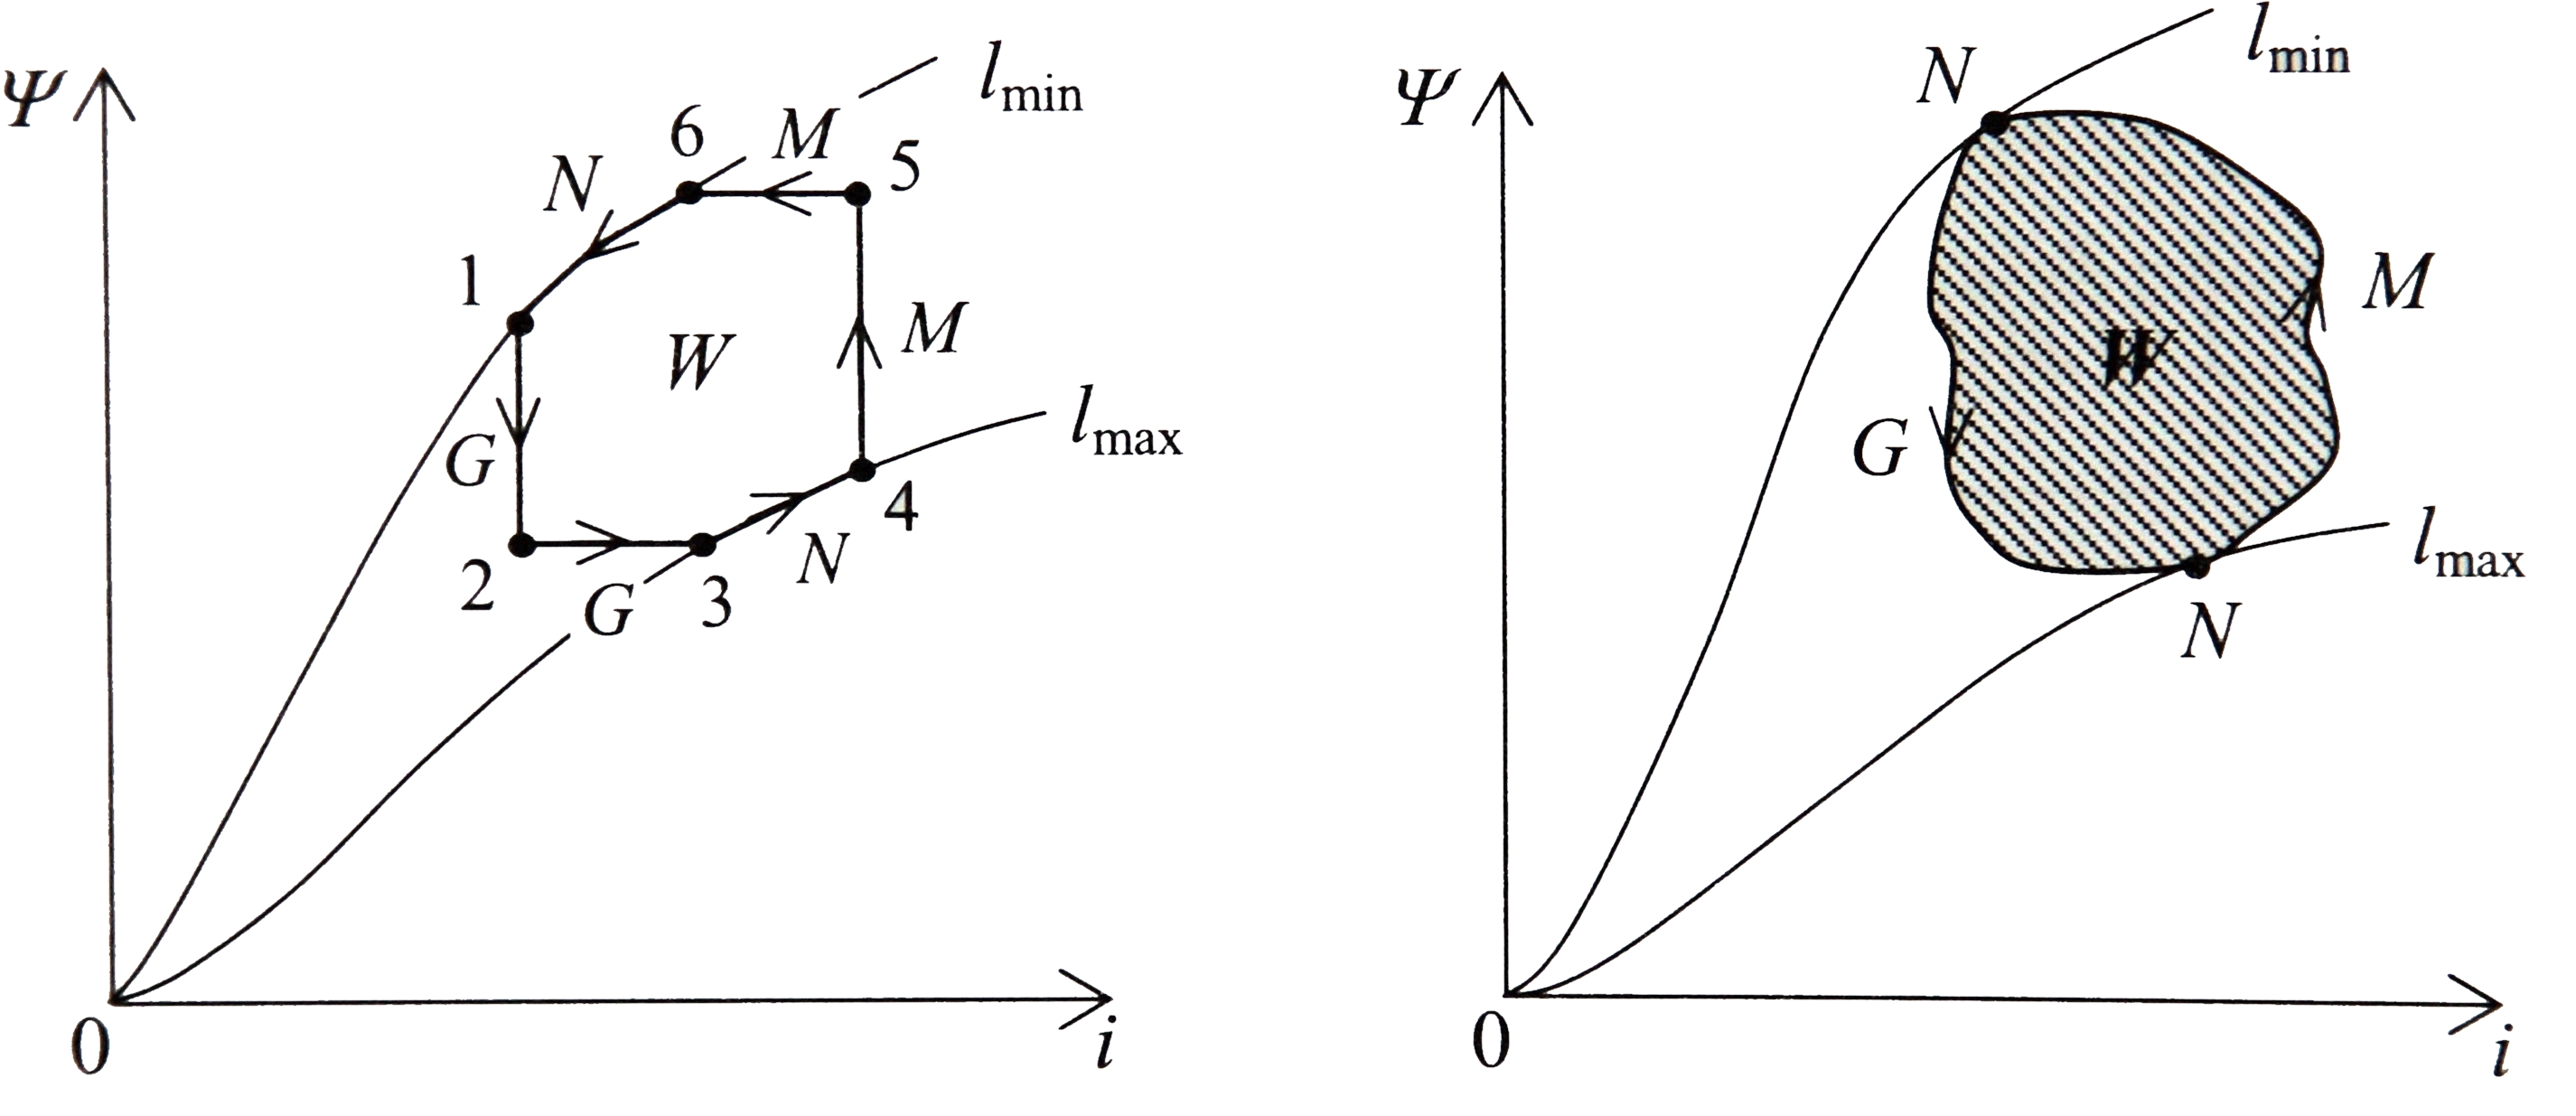
\includegraphics[width=0.9\linewidth]{teo_fig013.jpg}
        \caption{Elektromagnet jako reluktanční stroj. Plocha smyčky je rovna práci vykonané během
                 jednoho cyklu.
                 (\cite[s.~164]{Patocka4})}
        \label{teo:fig013}
      \end{figure}

      Po dokončení celého pracovního cyklu stroj vykonal užitečnou mechanickou práci \(W\), která 
      je rovna ploše pracovní smyčky. Jedná se o analogii hysterezní smyčky. V obou případech je 
      plocha smyčky rovna energii odebrané z napájecího zdroje. V případě stroje je tato energie 
      přeměněná na užitečnou energii mechanickou, v případě hystereze na neužitečnou energii 
      tepelnou. Na obr. \ref{teo:fig013} vpravo je ukázán příklad skutečného cyklu, plynule se 
      měnícího, ve kterém došlo ke zkrácení obou neutrálních neužitečných úseků \(N\) na pouhé body.

      \luagraphic[1]{teo_fig015.jpg}{Carnotův cyklus parního stroje. 
      (\cite[s.~165]{Patocka4})}{teo:fig015}

      Stejným způsobem probíhá cyklus točivého, tzv. spínaného reluktančního motoru \textbf{SRM}. Z 
      popisu cyklu je zřejmé, že v rámci jednoho uzavřeného cyklu musí stroj vystřídat vždy oba 
      režimy, tj. motorový i generátorový. To je jednoznačným důkazem, že takový stroj nemůže mít 
      nikdy hladký chod, jeho moment musí mít vždy pulsační charakter v rámci jedné otáčky. 
      Momentové pulsace nelze zcela odstranit ani zvyšováním počtu fází stroje, ani jiným způsobem, 
      např. úpravou regulačních algoritmů.

      Pro dokreslení fyzikálních souvislostí lze pracovní cyklus reluktančního stroje přirovnat ke 
      Carnotově\footnote{Nicohi Léonard Sadi Carnot (1796-1832), francouzský fyzik a vojenský 
      inženýr. Svou prací o tepelných strojích, publikovanou 1824, položil základy k formulací 
      druhé věty termodynamické.} cyklu stroje parního. Na obr. \ref{teo:fig015} se jedná o 
      závislost tlaku plynu na objemu. Křivky označené \(T_1\) \(T_2\) jsou \emph{izotermy}, křivky 
      \(A_1\), \(A_2\) jsou \emph{adiabaty}. \(W\) je mechanická práce, vykonaná během jednoho 
      pracovního cyklu.

      
    \subsection{Síla ve vzduchové mezeře elektromagnetu}
       O elektromagnetických silách pojednává podrobněji kapitola \ref{vol02:ES:sec11}.
       Elektromagnet podle obr. \ref{teo:fig014} je napájen z ideálního zdroje konstantního proudu.
       
      \begin{figure}[ht!] %\ref{teo:fig014}
        \centering
        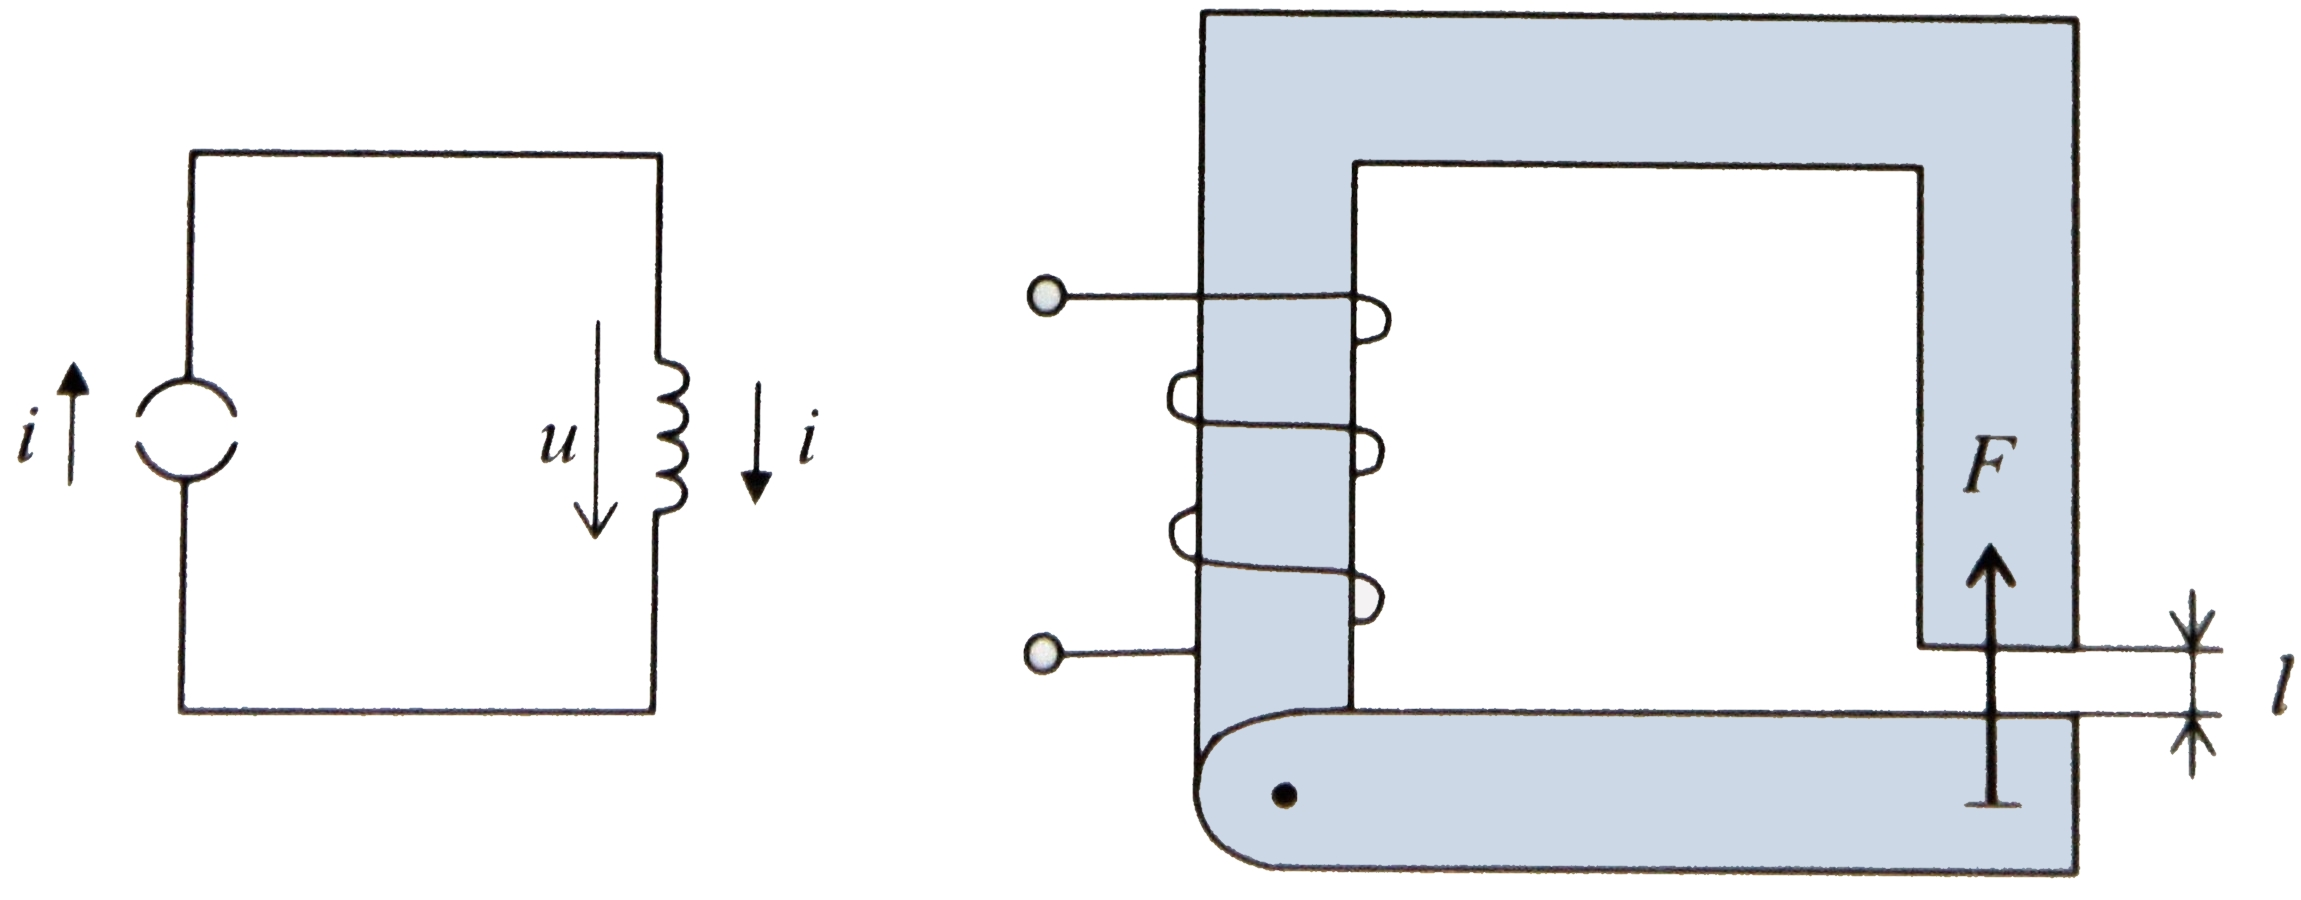
\includegraphics[width=0.8\linewidth]{teo_fig014.jpg}
        \caption{K odvození síly ve vzduchové mezeře elektromagnetu.
                 (\cite[s.~165]{Patocka4})}
        \label{teo:fig014}
      \end{figure}
      Při \emph{zkrácení} vzduchové mezery o diferenciální délku \(dl\) působí síla ve \emph{směru 
      pohybu}, a proto elektromagnet vykoná diferenciální mechanickou práci
      \begin{equation}\label{TEO:eq060}
        \dd{W_{mech}} = F\,dl.
      \end{equation}
      Tato diferenciální práce musí být kryta ze zdroje konstantního proudu \(i\), a to takovým 
      způsobem, aby celková energie soustavy zůstala zachována\footnote{Naopak, při prodloužení 
      mezery působí síla proti směru pohybu, proto elektromagnet mechanickou energii spotřebovává, 
      přeměňuje ji na elektrickou a odevzdává do napájecího zdroje. Tehdy se chová jako generátor}. 
      Odtud plyne, že součet diferenciálních energetických přírůstků v soustavě musí být nulový:
      \begin{equation}\label{TEO:eq061}
        \dd{W_{mech}} + dW = 0.
      \end{equation}
      Z rovnic (\ref{TEO:eq060}), (\ref{TEO:eq061}) lze určit velikost síly 
      \begin{equation}\label{TEO:eq062}
        F = \der{W_{mech}}{l} = - \der{W}{l},
      \end{equation}
      kde \(dW\) je přírůstek energie dodaný zdrojem proudu do magnetického obvodu elektromagnetu. 
      Protože magnetická vodivost železa je řádově větší než vodivost vzduchové mezery, lze vliv 
      železa zanedbat a předpokládat, že veškerá energie sídlí pouze ve vzduchové mezeře. V tom 
      případě magnetická mezera obvod výrazně \emph{linearizuje}, proto je možno určit energii 
      \(W\) magnetického pole z rovnice (\ref{TEO:eq027}): 
      \begin{equation}\label{TEO:eq064}
        W = \frac{1}{2}i^2L = \frac{1}{2}i^2N^2\mu_0\frac{S_{Fe}}{l},
      \end{equation}
      kde \(S_{Fe}\) je průřez železa, tedy i plocha vzduchové mezery. Sílu určíme tak, že do 
      rovnice (\ref{TEO:eq062}) dosadíme rovnici (\ref{TEO:eq064}):
      \begin{align}
        F = - \der{W}{l} 
         &= -\der{ }{l}\left(\frac{1}{2}i^2L\right)= -\frac{1}{2}i^2\der{ }{l}(L) \nonumber \\
         &= -\frac{1}{2}i^2\der{ }{l}\left(N^2\mu_0\frac{S_{Fe}}{l}\right)        \nonumber \\
         &=  \frac{1}{2}i^2\left(N^2\mu_0\frac{S_{Fe}}{l^2}\right)
          =  \frac{1}{2}i^2\frac{L}{l}.                                           \label{TEO:eq065}
      \end{align}
      Rovnici (\ref{TEO:eq065}) lze upravit do konečného tvaru
      \begin{subequations}
        \begin{align}  %\label{TEO:eq069}
           \Aboxed{F &= \frac{1}{2}i^2\frac{L}{l}    
                      = \frac{1}{2}\frac{i^2L^2}{Ll}
                      = \frac{1}{2}\frac{\Psi^2}{Ll}}                     \label{TEO:eq069a} \\
           \Aboxed{F &= \frac{1}{2}\frac{(NBS_{Fe})^2}{N^2\mu_0S_{Fe}}
                      = \frac{1}{2}\frac{B^2}{\mu_0}S_{Fe}}               \label{TEO:eq069b}
        \end{align}
      \end{subequations}
      Plošný mechanický tlak, vznikající ve vzduchové mezeře, má zřejmé velikost 
      \begin{equation}\label{TEO:eq068}
        \boxed{p = \frac{F}{S_{Fe}} = \frac{1}{2}\frac{B^2}{\mu_0}}\,, \qquad [Ns/m^2; T, H/m],
      \end{equation}
      Zdůrazníme, že se jedna o tlak sídlící v objemu vzduchové mezery (nikoli v železe).
      
    \subsection{Princip reciprocity u elektromagnetu}
      V kapitole \ref{vol02:teo:IchapIIsecIsubIX} bylo ukázáno, že princip reciprocity platí i u
      všech \emph{elektromechanických měničů} energie. Musí tedy platit i v případě elektromagnetu.
      Pohlížíme-li na elektromagnet jako na \uv{přenosový dvojbran} s elektrickými veličinami
      \(u(t)\), \(i(t)\) na elektrické bráně a s mechanickými veličinami \(F(t)\), \(v(t)\) na
      mechanické bráně, pak lze tento systém popsat hybridní H-maticí ve tvaru
      \begin{subequations}
      \label{TEO:eq075}
        \begin{align}
          u(t) &= Ri(t) + L_d[i,l]\der{i(t)}{t} + K_v[i,l]v(t),  \label{TEO:eq075a} \\
          F(t) &= - K_F[i,l]i(t) + -m_i\der{v(t)}{t},            \label{TEO:eq075b} 
        \end{align}
      \end{subequations}
      Napěťová rovnice vznikla doplněním rovnice (\ref{TEO:eq076}) o napěťový úbytek na odporu 
      vinutí. Záporná znaménka ve druhé rovnici jsou důsledkem toho, že síla \(F\) působí proti 
      kladnému smyslu zvětšující se dráhy \(l\). Veličina \(m_i\) je setrvačná hmotnost vlastního 
      elektromagnetu. Má-li platit princip reciprocity, musí platit \(K_v = - K_F\).
      
      \emph{Rychlostní převodní funkci} určíme jako parciální derivaci rovnice (\ref{TEO:eq075a}) 
      podle rychlosti: 
      \begin{align}
        K_v[i,l] &= \pder{u(t)}{v(t)} = \der{\Psi(t)}{t}\der{t}{l(t)}          
                  = \der{\Psi(t)}{l(t)}                                        \nonumber \\
                 &= \der{\Psi}{l} = i\der{L}{l}.\label{TEO:eq077} \\
        \shortintertext{Z rovnice (\ref{TEO:eq077}) plyne}
        K_v[i,l] &= i\der{L}{l} = i\der{ }{l}\left(N^2\mu_0\frac{S_{Fe}}{l}\right) 
                  = - i\left(N^2\mu_0\frac{S_{Fe}}{l^2}\right)                  \nonumber \\
                 &= -\frac{Bl}{\mu_0N}\left(N^2\mu_0\frac{S_{Fe}}{l^2}\right)
                  = - \frac{NBS_{Fe}}{l} \label{TEO:eq078}   \\ 
        \shortintertext{\emph{ Silovou převodní funkci} určíme jako parciální derivaci síly podle 
        proudu z rovnice (\ref{TEO:eq065}):}
        K_F[i,l] &= \pder{F}{i} = \pder{ 
        }{i}\left[\frac{1}{2}i^2\left(N^2\mu_0\frac{S_{Fe}}{l^2}\right)\right]  
                  = i\left(N^2\mu_0\frac{S_{Fe}}{l^2}\right)                    \nonumber \\
                 &= \frac{Bl}{\mu_0N}\left(N^2\mu_0\frac{S_{Fe}}{l^2}\right) 
                  = \frac{NBS_{Fe}}{l} \label{TEO:eq079}
      \end{align}
      Vidíme, že opravdu platí \(K_v = - K_F\), elektromagnet tedy vyhovuje principu reciprocity. 
      
    \subsection{Matematický model levitačního elektromagnetu}
      Levitační elektromagnet v uspořádání podle obr. \ref{teo:fig016} je využíván ke konstrukci 
      rychlovlaků, v jiném geometrickém uspořádání ke konstrukci magnetických ložisek. Jedná se o 
      tzv. \textbf{aktivní magnetickou levitaci\footnote{Magnetickou levitaci je možno realizovat i 
      na jiných fyzikálních principech, které nevyužívají zpětnovazební kybernetickou regulaci, 
      proto je lze souhrnně nazývat jako levitace \emph{pasivní}.}}, při které je 
      \emph{kybernetickou zpětnovazební regulační smyčkou udržována konstantní vzduchová mezera 
      mezi magnetem a kolejnici}. Z pohledu kybernetiky je magnet akčním členem a pracuje jako 
      lineární motor, konající práci při pohybu ve svislém směru. Volba souřadného systému 
      matematického modelu, tj. volba kladných směrů polohy, rychlosti, zrychlení a sil plyne z 
      obr. \ref{teo:fig016}. Síla \(F_r\) má význam libovolné rušivé dynamické síly, která může na 
      magnet působit
      
      \begin{figure}[ht!]  %\ref{teo:fig016}
        \centering
        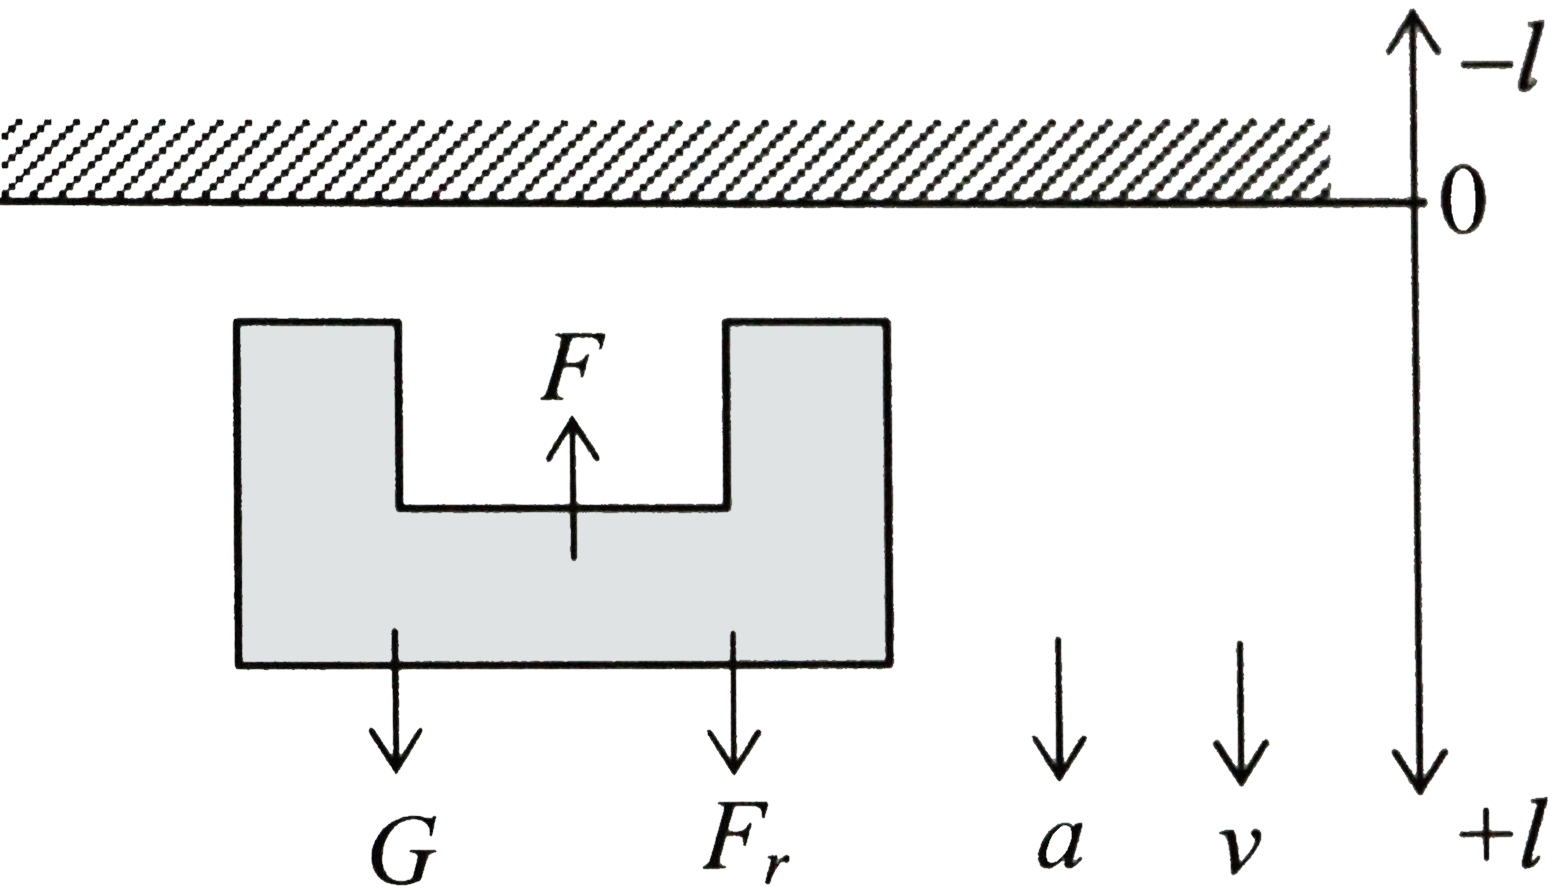
\includegraphics[width=0.6\linewidth]{teo_fig016.jpg}
        \caption{Základní uspořádání levitačního elektromagnetu.
                 (\cite[s.~16]{Patocka4})}
        \label{teo:fig016}
      \end{figure}
      Pro výslednou akcelerační sílu \(F_a\). tedy i pro výsledné zrychlení \(a\) zřejmé platí
      \begin{subequations}
      \label{TEO:eq063}
        \begin{align}
          F_a &= G + F_r - F,             \label{TEO:eq063a} \\
          ma  &= mg + F_r - F,            \label{TEO:eq063b} \\
          a   &= g + \frac{F_r -F}{m}.    \label{TEO:eq063c}
        \end{align}
      \end{subequations}
      Rychlost je integrálem ze zrychlení
      \begin{equation}\label{TEO:eq066}
        v(t) = v_0 + \int{a(t)\dd{t}}.
      \end{equation}
      Okamžitá poloha (délka vzduchové mezery) je integrálem z rychlosti
      \begin{equation}\label{TEO:eq067}
        l(t) = l_0 + \int{v(t)\dd{t}}.
      \end{equation}
      Sílu \(F\) elektromagnetu lze určit pomocí rovnice (\ref{TEO:eq069a} a \ref{TEO:eq069b}), je 
      však nutno zohlednit existenci dvou vzduchových mezer. Síly vznikají v obou mezerách, 
      výsledná síla je tedy dvojnásobná:
      \begin{equation}\label{TEO:eq070}
        F = 2\frac{1}{2}\frac{B^2}{\mu_0}S_{Fe} = \frac{B^2}{\mu_0}S_{Fe}.
      \end{equation}
      Pro svorkové napětí elektromagnetu platí rovnice
      \begin{equation}\label{TEO:eq071}
        u(t) = Ri(t) + \der{\Psi(t)}{t} = Ri(t) + NS_{Fe}\der{B(t)}{t}.
      \end{equation} 
      Integrací rovnice (\ref{TEO:eq071}) lze určit magnetickou indukci:
      \begin{equation}\label{TEO:eq072}
      B(t) = B_0 + \frac{1}{NS_{Fe}}\int\left[u(t) - Ri(t)\right]\dd{t},
      \end{equation}
      kde \(B_0\) je libovolná počáteční integrační konstanta. Celkové magnetické napětí 
      magnetického obvodu lze vyjádřit rovnici
      \begin{equation}\label{TEO:eq073}
      Ni = 2H_vl+H_{Fe}l_{Fe} = 2\frac{B}{\mu_0}l + H(B)l_{Fe},
      \end{equation}
      kde funkce \(H(B)\) je inverzní funkcí k magnetizační charakteristice \(B(H)\) použitého 
      železa. Z rovnice (\ref{TEO:eq073}) plyne
      \begin{equation}\label{TEO:eq074}
        i = \frac{2Bl}{N\mu_0} + \frac{l_{Fe}}{N}H(B).
      \end{equation}
      Matematický model levitačního elektromagnetu je pak dán souborem rovnic (\ref{TEO:eq063}), 
      (\ref{TEO:eq066}), (\ref{TEO:eq067}), (\ref{TEO:eq070}), (\ref{TEO:eq072}), 
      (\ref{TEO:eq074}). Realizace modelu v prostředí Matlab-Símulink je ukázána na obr. 
      \ref{teo:fig017}. V pravé částí obrázku je model magnetu doplněn o matematický model horního 
      a dolního dorazu, bez něhož by byl model nepoužitelný.
      
      \begin{figure*}[ht!] %\ref{teo:fig017}
        \centering
        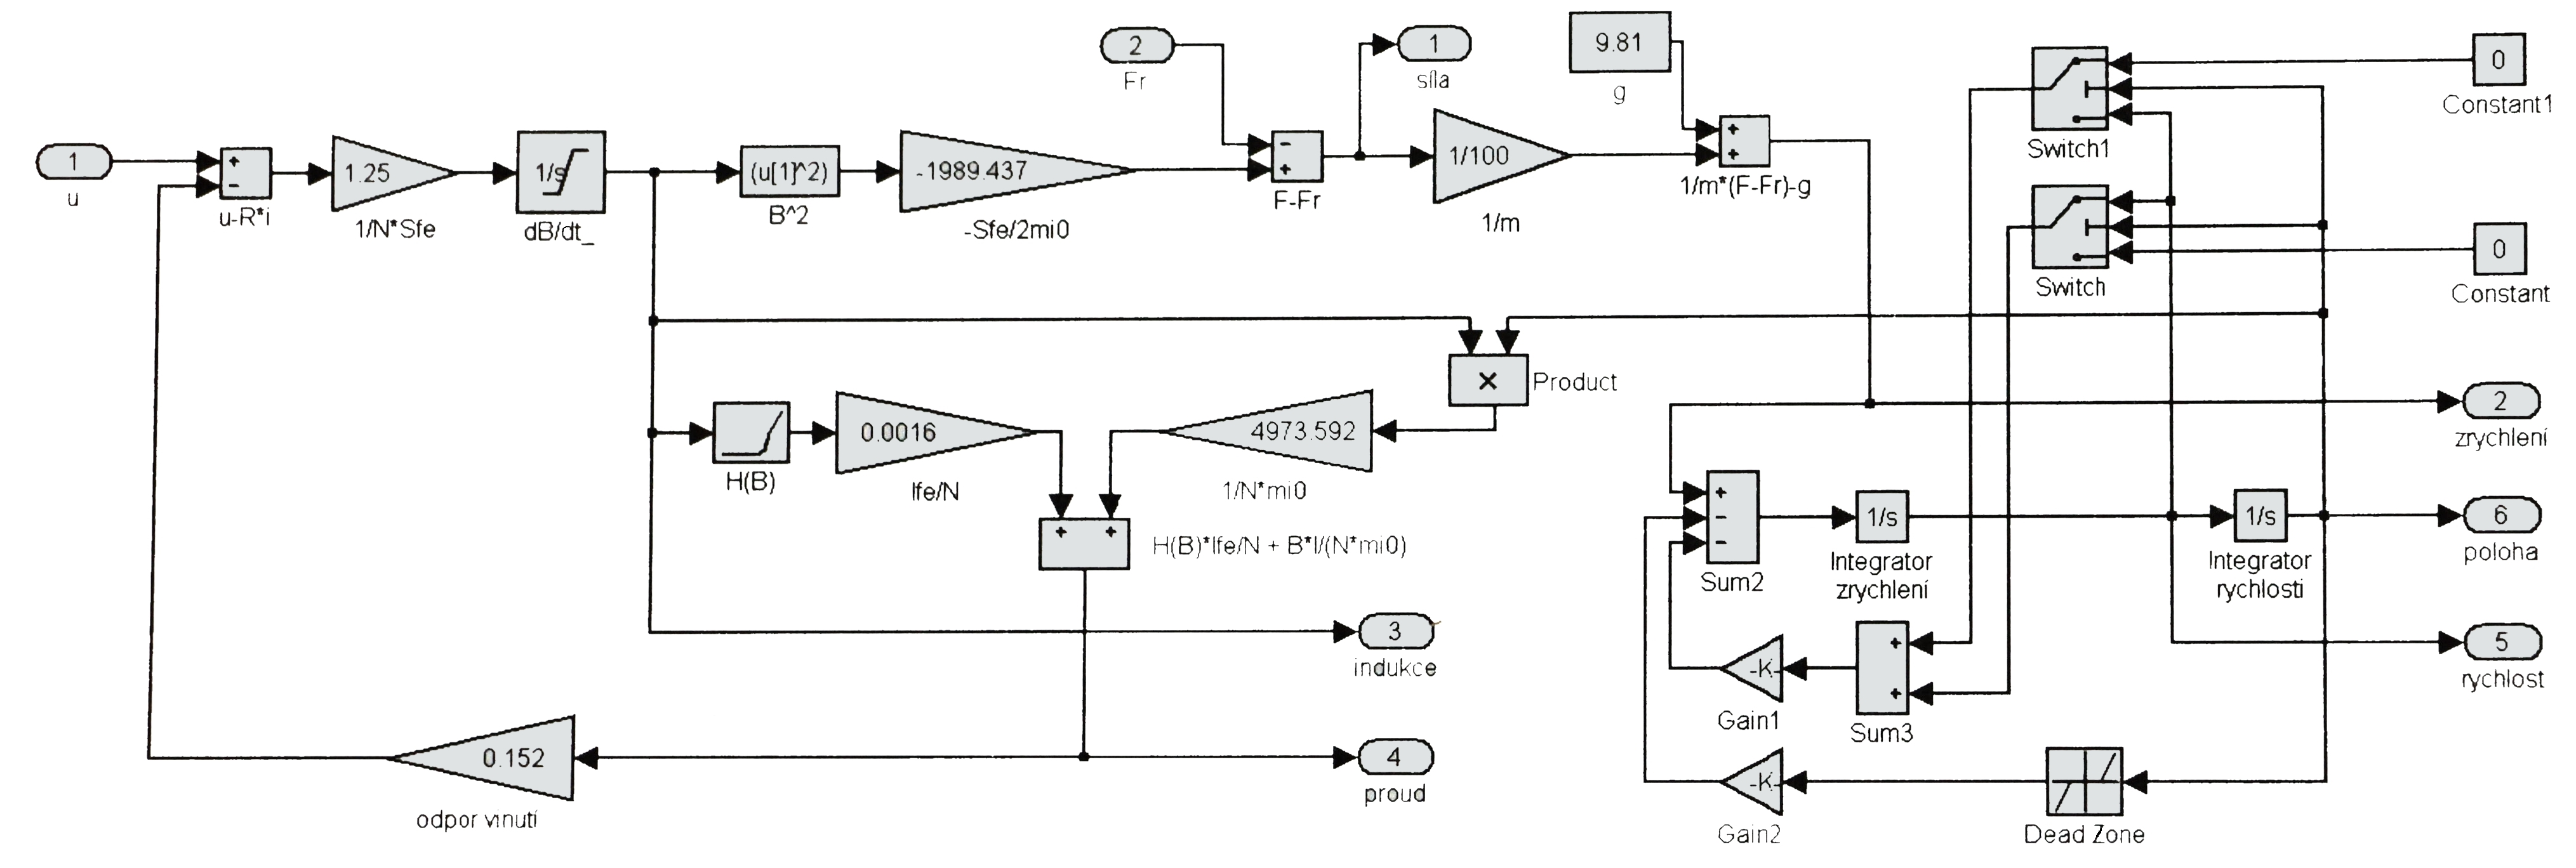
\includegraphics[width=0.9\linewidth]{teo_fig017.jpg}
        \caption{Matematický model levitačního elektromagnetu v prostředí Matlab-Simulink.
                 (\cite[s.~168]{Patocka4})}
        \label{teo:fig017}
      \end{figure*}

%} % tikzset
%~~~~~~~~~~~~~~~~~~~~~~~~~~~~~~~~~~~~~~~~~~~~~~~~~~~~~~~~~~~~~~~~~~~~~~~~~~~~~~~~~~~~~~~~~~~~~~~~~~